\chapter{分布族}
\label{chap:distribution-families}

一枚只会出现$0,1,2$三种结果的骰子，我们不知道它的概率表，只知道平均点数大约是$1$。满足这个条件的概率表有无穷多张，它们排成三角形里的一条线段。一台仪器的读数总是正的，平均为$1$，满足这一点的密度更多，多到无法用有限个数字逐一列出。在挑选“哪一个分布”之前，先要说清楚允许哪些分布，以及用什么样的参数给它们编号。

一旦用参数编号，就会出现新的问题。同一个分布可能被几组不同的参数表示，改变某个参数可能只是把分布挪动或拉伸，也可能改变它的形状、支撑甚至类型。本章研究构造和表示一组分布的几种常用办法，着重回答：改变参数时，什么保持不变，什么随之改变。

第一节先把“分布族”与“参数表示”分开，用概率表的三角形说明候选范围的含义，再把不同参数是否给出不同分布作为可辨识性问题提出。后面四节分别从四个方向构造分布族。推前构造固定一个基础随机变量，让映射随参数变化；混合分布让成分的选择本身随机；Copula把联合分布拆成各分量的边缘规律与它们之间的依赖；指数族对若干统计量施加指数权重，并用一个归一化函数把参数、矩与表示的冗余联系起来。

这四种构造并不互斥：同一个高斯族既是标准高斯的位置尺度变换，也是一个指数族，多元t分布既是正态尺度混合，也可以拆成t边缘加上它的Copula。本章只讨论怎样表示一族分布，以及参数是否唯一；在给定约束下选出哪一个分布、在族内怎样逼近给定分布，分别在第~\ref{chap:distribution-selection}章和第~\ref{chap:distribution-approximation}章研究。

\section{分布族与参数}
\label{sec:dfam-families}

回到章首那枚三面骰子。它的概率规律就是一张表$(p_0,p_1,p_2)$，三个数非负、和为$1$。在知道更多之前，这样的表都有可能；知道平均点数是$1$以后，只剩一部分表还有资格。这里有两件不同的事：一件是哪些概率规律被允许，另一件是怎样给被允许的规律编号。本节先讨论前者，再讨论后者，并说明编号时可能出现的重复。

\subsection{候选分布的范围}
\label{sec:dfam-candidates}

设$(\mathcal{X},\mathcal{F}_{\mathcal{X}})$是取值空间，记$\mathcal{P}(\mathcal{X})$为其上全体概率测度。研究一个随机现象时，我们往往不能断定它的分布是哪一个，只能根据机制和已知事实圈出一个范围。

\begin{definition}[分布族]
\label{def:dfam-family}
$\mathcal{P}(\mathcal{X})$的任一非空子集$\mathcal{C}$称为$\mathcal{X}$上的一个\term{分布族}（family of distributions）。
\end{definition}

分布族的成员是概率测度本身，不是随机变量，也不是参数。说“$X$的分布属于$\mathcal{C}$”，是在对$X$的概率规律提出要求，而不是在对$X$的取值或某个数字提出要求。下面先在有限取值空间上看这些要求长什么样。

\paragraph{有限概率表的三角形}
取$\mathcal{X}=\{0,1,2\}$。一个概率测度由三个数$p_x=P(\{x\})$确定，全体概率测度对应集合
\begin{equation}
  \Delta_2=\{(p_0,p_1,p_2):p_x\geq0,\ p_0+p_1+p_2=1\}.
  \label{eq:dfam-simplex}
\end{equation}
它是$\mathbb{R}^{3}$中以三个坐标向量为顶点的三角形，即第~\ref{chap:multivariate-distributions}章的标准单纯形。顶点是集中在一点的分布，三条边是恰有一个结果概率为零的分布，内部是三个结果都可能出现的分布。图~\ref{fig:dfam-simplex-candidates}把这个三角形摊平画出。

候选范围的第一类要求是固定支持。要求三个结果都有正概率，候选集合是三角形的内部；已知结果$2$不会出现，候选集合是$p_2=0$那条边。这类要求只看哪些点上有质量，不看质量有多少。

第二类要求是矩约束。要求$\mathbb{E}_P[X]=1$，就是
\[
  p_1+2p_2=1 .
\]
与$p_0+p_1+p_2=1$相减，得到
\[
  p_0=p_2 .
\]
所以满足约束的表形如$(t,1-2t,t)$，$0\leq t\leq1/2$，这是从顶点$(0,1,0)$到底边中点$(1/2,0,1/2)$的一条线段。均匀表$(1/3,1/3,1/3)$在线段上，点$(1/2,0,1/2)$也在线段上，它把一半质量放在$0$、一半放在$2$，平均同样是$1$。

\begin{BookInlineFigure}
  \centering
  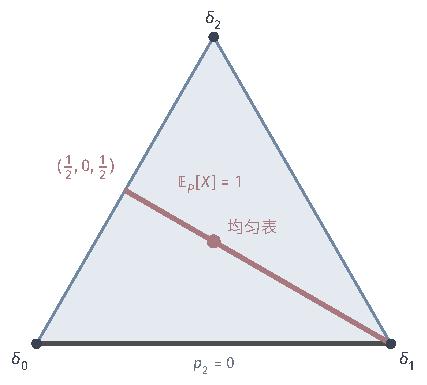
\includegraphics[width=72.4mm]{figures/07-probability/04-distribution-analysis/tikz/dfam-simplex-candidates/figure.pdf}
  \caption{$\{0,1,2\}$上的全体概率表构成三角形$\Delta_2$，三个顶点是点质量$\delta_0,\delta_1,\delta_2$。浅蓝区域是三个结果都有正概率的内部；深灰粗边$p_2=0$是不出现结果$2$的表，也是相对计数测度$\nu$（支撑$\{0,1\}$）绝对连续的表；红色线段是满足$\mathbb{E}_P[X]=1$的表$(t,1-2t,t)$，红点为均匀表。}
  \label{fig:dfam-simplex-candidates}
\end{BookInlineFigure}

第三类要求是相对某个\term{参考测度}（reference measure）$\nu$绝对连续，即凡$\nu(B)=0$的集合都有$P(B)=0$。在$\{0,1,2\}$上取$\nu$为$\{0,1\}$上的计数测度，$\nu(\{2\})=0$，于是$P\ll\nu$恰好意味着$p_2=0$，与固定支持的要求相同。在有限空间上两者没有差别；在连续空间上，绝对连续才保证密度$\mathrm{d}P/\mathrm{d}\nu$存在（Radon–Nikodym定理，见\BookChapterRef{chap:measure-densities}{卷四第8章“测度的密度”}），它是用密度描述分布族的前提。

几类要求可以叠加。同时要求三个结果都可能出现、平均为$1$，候选集合就是去掉两个端点的开线段。每加一条要求，三角形里剩下的部分就小一些，但它仍然是概率表的集合，我们还没有给其中的表起任何名字。

\paragraph{给定均值的密度}
换到连续情形，差别就显出来了。设读数取值于$(0,\infty)$，要求分布相对Lebesgue测度绝对连续且均值为$1$，候选集合是
\begin{equation}
  \mathcal{C}_1=\Bigl\{f\geq0:\int_0^\infty f(x)\,\mathrm{d}x=1,\ \int_0^\infty xf(x)\,\mathrm{d}x=1\Bigr\}.
  \label{eq:dfam-mean-one}
\end{equation}
这里两个密度若几乎处处相等，就看作同一个分布。$\operatorname{Exp}(1)$的密度$\mathrm{e}^{-x}$、$\operatorname{Gamma}(2,2)$的密度$4x\mathrm{e}^{-2x}$和$\operatorname{Unif}(0,2)$的密度$1/2$（$0<x<2$）都在$\mathcal{C}_1$里，形状却各不相同，见图~\ref{fig:dfam-mean-one-densities}。点质量$\delta_1$的均值也是$1$，但它不相对Lebesgue测度绝对连续，被第一个要求排除在外。

\begin{BookInlineFigure}
  \centering
  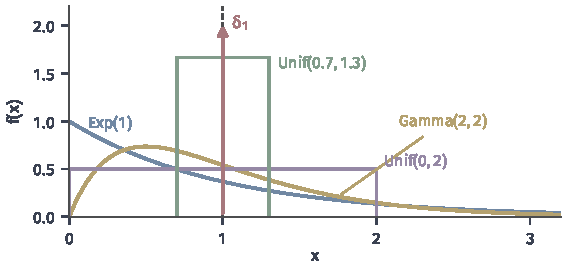
\includegraphics[width=96mm]{figures/07-probability/04-distribution-analysis/matplotlib/dfam-mean-one-densities/figure.pdf}
  \caption{均值都等于$1$的几个分布。蓝线为$\operatorname{Exp}(1)$，黄线为$\operatorname{Gamma}(2,2)$，紫线为$\operatorname{Unif}(0,2)$，绿线为$(1-a,1+a)$上的均匀密度（$a=0.3$）；红色箭头表示点质量$\delta_1$，它没有相对Lebesgue测度的密度。深灰竖线标出均值$x=1$。}
  \label{fig:dfam-mean-one-densities}
\end{BookInlineFigure}

$\mathcal{C}_1$大到什么程度？取$0<a_1<a_2<\cdots<a_n<1$，令$g_k$为区间$(1-a_k,1+a_k)$上的均匀密度。区间关于$1$对称，所以每个$g_k$的均值都是$1$。对任意权重$c_k\geq0$、$\sum_kc_k=1$，凸组合$\sum_kc_kg_k$仍非负、积分为$1$、均值为$1$，所以它也在$\mathcal{C}_1$中。

这$n$个密度线性无关。设$\sum_kc_kg_k=0$几乎处处成立。在区间$(1+a_{n-1},1+a_n)$上只有$g_n$不为零，所以$c_n=0$；去掉$g_n$后对$g_{n-1}$重复同样的论证，依次得到所有$c_k=0$。由于$n$可以任意大，$\mathcal{C}_1$不包含在任何有限维仿射子空间中，因而不能写成有限个固定密度带参数的线性组合。

这说明候选范围与参数表示是两回事。三角形上的线段可以用一个数$t$编号，$\mathcal{C}_1$却不能用有限个系数作线性编号。描述候选集合时不应预设它总有一个有限维参数；有限维的参数族是从候选集合中再挑出的一部分，挑法正是本章后面几节的内容。

\subsection{参数表示与可辨识性}
\label{sec:dfam-identifiability}

给分布编号，就是指定一个集合$\Theta$和一个映射$\bm{\theta}\mapsto P_{\bm{\theta}}$，让每个参数值对应一个概率测度。

\begin{definition}[参数化分布族]
\label{def:dfam-parametric-family}
设$\Theta$是一个集合，对每个$\bm{\theta}\in\Theta$给定$P_{\bm{\theta}}\in\mathcal{P}(\mathcal{X})$。分布族$\{P_{\bm{\theta}}:\bm{\theta}\in\Theta\}$称为以$\Theta$为\term{参数空间}（parameter space）的参数化分布族。若各$P_{\bm{\theta}}$都相对同一个参考测度$\nu$绝对连续，记其密度为$p_{\bm{\theta}}$。
\end{definition}

分布族是映射的像，参数化是映射本身。同一个族可以有许多参数化。Bernoulli族$\{\operatorname{Bern}(p):0<p<1\}$可以直接用$p$编号，也可以用$\eta\in\mathbb{R}$编号：
\[
  p=\frac{\mathrm{e}^{\eta}}{1+\mathrm{e}^{\eta}} .
\]
两种编号得到的分布集合完全相同，对应单纯形$\Delta_1$（一条线段）去掉两个端点，差别只在刻度：$p$在$(0,1)$上均匀刻度，$\eta$把靠近$0$和$1$的部分拉长到整条实轴。

\paragraph{重复的参数}
编号可能是冗余的。令$(a,b)\in(0,\infty)^2$对应$\operatorname{Bern}\bigl(a/(a+b)\bigr)$。$(1,2)$与$(2,4)$给出同一个分布$\operatorname{Bern}(1/3)$；更一般地，从原点出发的每条射线$\{(ca,cb):c>0\}$整条对应同一个分布，如图~\ref{fig:dfam-redundant-parameters}。两个参数，却只描述一个自由度的分布。

\begin{BookInlineFigure}
  \centering
  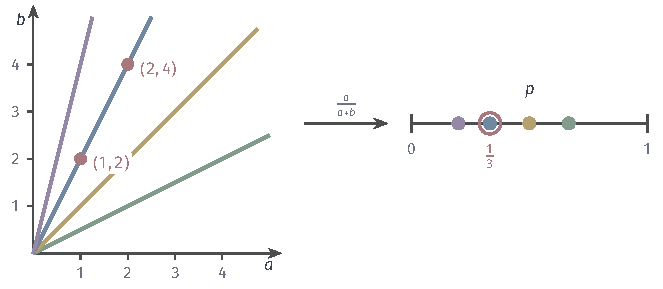
\includegraphics[width=112mm]{figures/07-probability/04-distribution-analysis/tikz/dfam-redundant-parameters/figure.pdf}
  \caption{冗余参数化$(a,b)\mapsto\operatorname{Bern}(a/(a+b))$。左：参数平面中，同一条射线上的点（同色）对应同一个分布，红点$(1,2)$与$(2,4)$都给出$\operatorname{Bern}(1/3)$。右：分布只由$p=a/(a+b)$决定，射线被压成线段$(0,1)$上的一点。}
  \label{fig:dfam-redundant-parameters}
\end{BookInlineFigure}

\begin{definition}[可辨识性]
\label{def:dfam-identifiable}
若对$\bm{\theta},\bm{\theta}'\in\Theta$，由$P_{\bm{\theta}}=P_{\bm{\theta}'}$总能推出$\bm{\theta}=\bm{\theta}'$，则称参数化$\bm{\theta}\mapsto P_{\bm{\theta}}$是\term{可辨识}（identifiable）的。
\end{definition}

可辨识就是参数到分布的映射是单射。这里的“分布相等”指两个概率测度在每个可测集上相等；用密度描述时，指$p_{\bm{\theta}}=p_{\bm{\theta}'}$相对$\nu$几乎处处成立。$\operatorname{Unif}[0,\theta]$与$\operatorname{Unif}(0,\theta)$的密度只在两个端点不同，它们是同一个分布，改动零测集上的值不产生新的参数。

可辨识性是参数化的性质，不是分布族的性质。上面的$(a,b)$参数化不可辨识，同一个Bernoulli族用$p$编号却可辨识。另一个常见的冗余来自参数只以组合形式出现：$(\theta_1,\theta_2)\mapsto\mathcal{N}(\theta_1+\theta_2,1)$中，直线$\theta_1+\theta_2=c$上的所有参数都给出$\mathcal{N}(c,1)$，分布只看得见和，看不见两个加数各是多少。

\paragraph{标签置换}
第~\ref{chap:random-vectors}章的混合分布带来另一种冗余。把两个高斯成分按权重相加，参数是$(w,\mu_1,\mu_2)$：
\[
  P_{(w,\mu_1,\mu_2)}=w\,\mathcal{N}(\mu_1,1)+(1-w)\,\mathcal{N}(\mu_2,1).
\]
交换两个成分的名字，得到
\[
  P_{(0.3,-1,2)}=P_{(0.7,2,-1)} .
\]
两组参数不同，分布却相同，这称为\term{标签置换}（label switching）。图~\ref{fig:dfam-label-switching}在$w=1/2$时画出$(\mu_1,\mu_2)$平面：关于对角线对称的两点给出同一个分布。

\begin{BookInlineFigure}
  \centering
  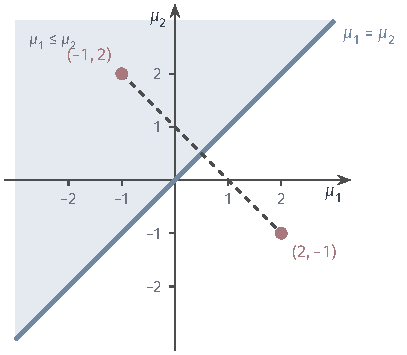
\includegraphics[width=68.9mm]{figures/07-probability/04-distribution-analysis/tikz/dfam-label-switching/figure.pdf}
  \caption{等权两成分高斯混合$\frac12\mathcal{N}(\mu_1,1)+\frac12\mathcal{N}(\mu_2,1)$的参数平面。关于对角线$\mu_1=\mu_2$对称的两点（红点$(-1,2)$与$(2,-1)$）给出同一个分布。限制在浅蓝的半平面$\mu_1\leq\mu_2$中，每个分布只剩一个参数。}
  \label{fig:dfam-label-switching}
\end{BookInlineFigure}

消除这种冗余有两个办法。一是缩小参数空间，例如只保留$\mu_1\leq\mu_2$的参数；二是承认参数只能确定到某种等价，把互相置换的参数看作同一个。两种办法都不改变分布族，只改变编号方式。混合表示中还有更多冗余，第~\ref{sec:dfam-mixture-nonuniqueness}节专门处理。

\paragraph{可辨识与能否从样本分辨}
可辨识性只问两个参数是否给出不同的分布，不问这种差别有多大。$\operatorname{Bern}(0.50)$与$\operatorname{Bern}(0.51)$是两个不同的分布，$p$参数化可辨识；可是各抛$100$次，正面次数的均值分别是$50$与$51$，标准差都约为$5$，两组次数的波动远大于均值之差，看一次试验结果几乎无法判断是哪一个。

另一个例子是$\theta\mapsto\mathcal{N}(\theta^{3},1)$。$\theta\mapsto\theta^{3}$是单射，所以它可辨识；但$\theta=0.1$与$\theta=0$对应的均值只差$0.001$，参数在$0$附近的变化几乎不改变分布。可辨识是分布层面的唯一性，是能否从数据推断参数的前提，但不是充分条件；有限样本下能多准确地估计参数，属于统计推断的问题，见\BookChapterRef{chap:parametric-statistical-inference}{卷八第1章“参数化统计推断”}。


\section{推前构造}
\label{sec:dfam-pushforward}

生成一个$\mathcal{N}(\mu,\sigma^{2})$样本，最省事的做法是先生成标准高斯$Z$，再计算$\mu+\sigma Z$。参数没有进入随机性，只进入了最后那一步计算。把这个做法一般化，就得到构造分布族的第一种办法：随机性由一个固定的基础分布提供，参数只控制把基础样本送到哪里去的映射。

设$(\mathcal{Z},\mathcal{F}_{\mathcal{Z}})$上有一个固定的概率测度$P_0$，$Z\sim P_0$。对每个参数$\bm{\theta}\in\Theta$给定可测映射$T_{\bm{\theta}}:\mathcal{Z}\to\mathcal{X}$，令$X_{\bm{\theta}}=T_{\bm{\theta}}(Z)$。由第~\ref{chap:probability-spaces}章，$X_{\bm{\theta}}$的分布是推前测度$P_{\bm{\theta}}=T_{\bm{\theta}\#}P_0$，即对每个$B\in\mathcal{F}_{\mathcal{X}}$，
\begin{equation}
  P_{\bm{\theta}}(B)=P_0\bigl(T_{\bm{\theta}}^{-1}(B)\bigr).
  \label{eq:dfam-pushforward}
\end{equation}

\begin{definition}[推前族]
\label{def:dfam-pushforward-family}
固定基础分布$P_0$与一族可测映射$\{T_{\bm{\theta}}:\bm{\theta}\in\Theta\}$，由式~\eqref{eq:dfam-pushforward}给出的$\{P_{\bm{\theta}}:\bm{\theta}\in\Theta\}$称为由$P_0$生成的\term{推前族}（pushforward family）。
\end{definition}

用单位质量的图景看，$P_0$把一份质量铺在$\mathcal{Z}$上，$T_{\bm{\theta}}$把每一小份质量搬到它在$\mathcal{X}$中的像；搬完以后落在$B$中的质量，就是原来落在$T_{\bm{\theta}}^{-1}(B)$中的质量。图~\ref{fig:dfam-pushforward-scheme}画出这个结构：基础分布固定，参数只出现在映射上。

\begin{BookInlineFigure}
  \centering
  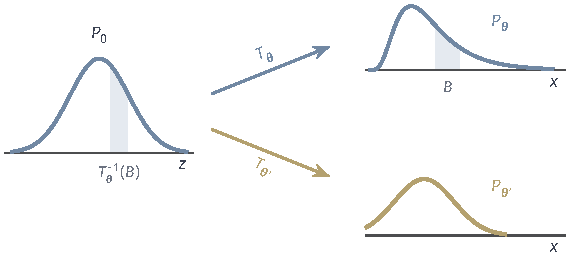
\includegraphics[width=96.6mm]{figures/07-probability/04-distribution-analysis/tikz/dfam-pushforward-scheme/figure.pdf}
  \caption{推前族的结构。左：固定的基础分布$P_0$，浅蓝带是集合$T_{\bm{\theta}}^{-1}(B)$；中间：随参数变化的映射$T_{\bm{\theta}}$；右：输出分布$P_{\bm{\theta}}$，浅蓝带是$B$。两块浅蓝区域的概率相等。两个参数$\bm{\theta}$、$\bm{\theta}'$（蓝、黄）共用同一个$P_0$。}
  \label{fig:dfam-pushforward-scheme}
\end{BookInlineFigure}

这种描述有两个直接的好处。第一，期望可以在基础空间上计算：对使下式一端有意义的可测函数$g$，
\begin{equation}
  \mathbb{E}_{P_{\bm{\theta}}}[g]=\mathbb{E}\bigl[g\bigl(T_{\bm{\theta}}(Z)\bigr)\bigr],
  \label{eq:dfam-pushforward-expectation}
\end{equation}
这是推前测度的积分公式，见\BookChapterRef{chap:pushforward-measures}{卷四第9章“推前测度”}。第二，生成样本只需生成$Z$再算一次映射。两者都不要求$P_{\bm{\theta}}$有密度。

推前构造的表达能力很强。第~\ref{chap:random-variables}章证明，若$U\sim\operatorname{Unif}(0,1)$，$Q$是任一分布函数$F$的分位数函数，则$Q(U)$的分布函数是$F$。所以$\mathbb{R}$上每一个分布都是$\operatorname{Unif}(0,1)$的推前。真正限制一个推前族的，是允许的映射类；下面两小节分别看最简单的映射类，以及映射怎样改变分布的结构。

\subsection{位置尺度族}
\label{sec:dfam-location-scale}

最简单的映射是平移加正向伸缩。第~\ref{chap:common-distributions}章已经用它解释过位置参数与尺度参数，这里把它作为推前族整理一遍，看分布函数、分位数和矩怎样随参数变化。

\begin{definition}[位置尺度族]
\label{def:dfam-location-scale}
设$Z$是实值随机变量，分布为$P_0$。对$\mu\in\mathbb{R}$、$\sigma>0$，令$P_{\mu,\sigma}$为$\mu+\sigma Z$的分布。$\{P_{\mu,\sigma}:\mu\in\mathbb{R},\ \sigma>0\}$称为由$P_0$生成的\term{位置尺度族}（location-scale family）。
\end{definition}

\paragraph{分布函数与分位数}
记$X=\mu+\sigma Z$。由$\sigma>0$，事件$\{X\leq x\}$与$\{Z\leq(x-\mu)/\sigma\}$相同，所以
\begin{equation}
  F_X(x)=F_Z\Bigl(\frac{x-\mu}{\sigma}\Bigr).
  \label{eq:dfam-ls-cdf}
\end{equation}
分布函数的图像只是被横向平移和伸缩。分位数函数的变化方向相反：第~\ref{chap:random-variables}章对$a>0$证明了$aZ+b$的分位数函数是$aQ_Z+b$，取$a=\sigma$、$b=\mu$，得到
\begin{equation}
  Q_X(u)=\mu+\sigma Q_Z(u),\qquad 0<u<1 .
  \label{eq:dfam-ls-quantile}
\end{equation}

式~\eqref{eq:dfam-ls-quantile}对每个$u$都成立，所以中位数、四分位数这些分位数一起按同一个仿射映射变化，四分位距乘以$\sigma$。把$X$的分位数对$Z$的同一水平分位数作图，点$(Q_Z(u),Q_X(u))$全部落在斜率为$\sigma$、截距为$\mu$的直线上。这条直线是检验“$X$是否属于$P_0$生成的位置尺度族”的图形办法，它不需要任何矩存在。

\paragraph{矩与标准化形状}
若$\mathbb{E}\lvert Z\rvert^{k}<\infty$，由凸函数$t\mapsto\lvert t\rvert^{k}$（$k\geq1$）的Jensen不等式，
\[
  \lvert X\rvert^{k}\leq2^{k-1}\bigl(\lvert\mu\rvert^{k}+\sigma^{k}\lvert Z\rvert^{k}\bigr),
\]
所以$X$的$k$阶矩也有限。由期望的线性和方差的缩放规律，
\begin{equation}
  \mathbb{E}[X]=\mu+\sigma\,\mathbb{E}[Z],\qquad\operatorname{Var}(X)=\sigma^{2}\operatorname{Var}(Z).
  \label{eq:dfam-ls-moments}
\end{equation}
矩不存在时，这些式子没有意义，但式~\eqref{eq:dfam-ls-cdf}与式~\eqref{eq:dfam-ls-quantile}照样成立。

再看偏度与峰度这类描述形状的量。设$\operatorname{Var}(Z)>0$，记$m_Z=\mathbb{E}[Z]$，$s_Z$为$Z$的标准差。由式~\eqref{eq:dfam-ls-moments}，$X$的标准化变量是
\[
  \frac{X-\mathbb{E}[X]}{\sqrt{\operatorname{Var}(X)}}=\frac{\sigma(Z-m_Z)}{\sigma s_Z}=\frac{Z-m_Z}{s_Z} .
\]
它与$\mu,\sigma$无关，所以只要相应的矩存在，标准化后的各阶矩，特别是偏度与峰度，在整个位置尺度族中保持不变。

更直接地，$(X-\mu)/\sigma=Z$，把族中任一成员按自己的参数标准化，都回到同一个基础分布。位置与尺度只决定分布放在哪里、铺开多宽，不改变标准化后的形状。

\paragraph{密度}
若$Z$有密度$f_Z$，第~\ref{chap:common-distributions}章已经算出$X$的密度
\begin{equation}
  f_X(x)=\frac{1}{\sigma}\,f_Z\Bigl(\frac{x-\mu}{\sigma}\Bigr).
  \label{eq:dfam-ls-density}
\end{equation}
因子$1/\sigma$来自伸缩：质量不变而区间拉长$\sigma$倍，单位长度上的质量就降为$1/\sigma$。

\paragraph{一个完整的例子}
取基础分布$Z\sim\operatorname{Exp}(1)$。由式~\eqref{eq:dfam-ls-cdf}，$X=\mu+\sigma Z$的分布函数是
\[
  F_X(x)=1-\exp\Bigl(-\frac{x-\mu}{\sigma}\Bigr),\qquad x\geq\mu ,
\]
$x<\mu$时为$0$。它的支撑是$[\mu,\infty)$，左端点随位置参数移动。$Z$的分位数函数是$Q_Z(u)=-\ln(1-u)$，由式~\eqref{eq:dfam-ls-quantile}，
\[
  Q_X(u)=\mu-\sigma\ln(1-u).
\]

取$\mu=1$、$\sigma=2$。中位数与两个四分位数分别是
\[
  Q_X(\tfrac12)=1+2\ln2\approx2.386,\quad Q_X(\tfrac14)\approx1.575,\quad Q_X(\tfrac34)\approx3.773 .
\]
四分位距是$2(\ln4-\ln\tfrac43)=2\ln3\approx2.197$，正好是$Z$的四分位距$\ln3$的$\sigma=2$倍。由式~\eqref{eq:dfam-ls-moments}，均值与方差是
\[
  \mathbb{E}[X]=1+2\cdot1=3,\qquad\operatorname{Var}(X)=4\cdot1=4 .
\]
$\operatorname{Exp}(1)$的偏度是$2$，所以族中每个成员的偏度都是$2$。

图~\ref{fig:dfam-location-scale}(a)画出三组参数的密度，它们看上去宽窄、位置都不同；(b)是分位数对照，三条曲线都是直线，斜率与截距读出$\sigma$与$\mu$。直线的事实说明它们属于同一个位置尺度族，宽窄的差别只是刻度的差别。

\begin{BookInlineFigure}
  \centering
  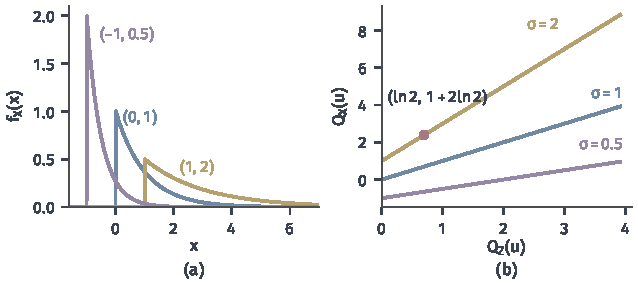
\includegraphics[width=108mm]{figures/07-probability/04-distribution-analysis/matplotlib/dfam-location-scale/figure.pdf}
  \caption{由$\operatorname{Exp}(1)$生成的位置尺度族。(a)$(\mu,\sigma)=(0,1)$（蓝）、$(1,2)$（黄）、$(-1,0.5)$（紫）的密度，支撑的左端点在$x=\mu$。(b)各成员的分位数$Q_X(u)$对基础分位数$Q_Z(u)$作图，$u$取$0.02$到$0.98$，得到斜率$\sigma$、截距$\mu$的直线；红点是$(\mu,\sigma)=(1,2)$的中位数$(\ln2,\ 1+2\ln2)$。}
  \label{fig:dfam-location-scale}
\end{BookInlineFigure}

\paragraph{基础分布的约定与参数的唯一性}
同一个位置尺度族可以由不同的基础分布生成。$\mathcal{N}(0,1)$与$\mathcal{N}(0,4)$生成的族都是全体高斯分布，但在后一种约定下，$\mu+\sigma Z$的标准差是$2\sigma$，同一个数字$\sigma$表示的宽度不同。一般地，$P_0$换成$a+bZ$（$b>0$）的分布，生成的族不变，参数按$(\mu,\sigma)\mapsto(\mu-\sigma a/b,\ \sigma/b)$换算。所以谈论位置和尺度参数的数值时，必须先固定基础分布。

固定基础分布以后，若$Z$不是几乎必然的常数，参数$(\mu,\sigma)$就是可辨识的。这时$Q_Z$不是常函数，可以取$u<v$使$Q_Z(u)<Q_Z(v)$。若$P_{\mu,\sigma}=P_{\mu',\sigma'}$，两者的分位数函数相同，由式~\eqref{eq:dfam-ls-quantile}，
\[
  \mu+\sigma Q_Z(u)=\mu'+\sigma'Q_Z(u),\qquad\mu+\sigma Q_Z(v)=\mu'+\sigma'Q_Z(v).
\]
两式相减得$(\sigma-\sigma')(Q_Z(v)-Q_Z(u))=0$，于是$\sigma=\sigma'$，再代回得$\mu=\mu'$。若$Z$是常数$c$，则$P_{\mu,\sigma}=\delta_{\mu+\sigma c}$，只有和$\mu+\sigma c$可见，参数不可辨识，这正是上一节$\mathcal{N}(\theta_1+\theta_2,1)$那类冗余的极端情形。

\paragraph{没有矩的成员}
Cauchy分布$f_Z(z)=1/(\pi(1+z^{2}))$没有均值。它生成的位置尺度族中，$\mu$不是均值，$\sigma$也不是标准差，但由$F_Z(z)=\tfrac12+\tfrac1\pi\arctan z$得$Q_Z(\tfrac14)=-1$、$Q_Z(\tfrac34)=1$，再由式~\eqref{eq:dfam-ls-quantile}，$\mu$是中位数，四分位距是$2\sigma$。位置尺度族的定义本身只用到映射，矩只是在存在时顺带跟着变化。

这个族的局限也很清楚：它永远改变不了标准化后的形状。由$\mathcal{N}(0,1)$生成的族里没有偏斜的分布，由$\operatorname{Exp}(1)$生成的族里偏度永远是$2$。要改变形状，映射必须不再是仿射的。

\subsection{映射对分布结构的影响}
\label{sec:dfam-map-effects}

仿射映射只做平移和伸缩。一般映射可以把基础分布弯曲、压扁或切碎，相应地改变输出分布的形状、支撑的维数，甚至让连续分布长出点质量。下面依次看三类映射：可逆的非线性映射、降低维数的映射和离散化。

\paragraph{可逆非线性映射改变形状}
取基础变量$Z\sim\mathcal{N}(0,1)$与映射$T_{\mu,\sigma}(z)=\exp(\mu+\sigma z)$，$\sigma>0$。它是$\mathcal{N}(0,1)$生成的位置尺度族再接一个固定的指数函数，输出是第~\ref{chap:random-variable-transformations}章的对数正态分布。指数函数把$\mathbb{R}$一一地送到$(0,\infty)$，导数处处为正，所以可以用一元单调换元公式求密度：
\[
  f_X(x)=\frac{1}{\sigma x}\,\varphi\Bigl(\frac{\ln x-\mu}{\sigma}\Bigr),\qquad x>0 .
\]

参数的角色在这里发生了变化。$X=\mathrm{e}^{\mu}\,(\mathrm{e}^{Z})^{\sigma}$，原来的位置参数$\mu$变成乘法因子$\mathrm{e}^{\mu}$，即对数正态族的尺度参数；原来的尺度参数$\sigma$成了指数$(\mathrm{e}^{Z})^{\sigma}$中的幂次，它改变的是形状。由高斯的矩母函数，
\[
  \mathbb{E}[X^{k}]=\mathrm{e}^{k\mu}\,\mathbb{E}[\mathrm{e}^{k\sigma Z}]=\mathrm{e}^{k\mu+k^{2}\sigma^{2}/2}.
\]
把$k=1,2,3$代入偏度的定义，因子$\mathrm{e}^{\mu}$全部约去，得到对数正态分布的偏度
\[
  (\mathrm{e}^{\sigma^{2}}+2)\sqrt{\mathrm{e}^{\sigma^{2}}-1},
\]
$\sigma=0.25$时约为$0.78$，$\sigma=1$时约为$6.18$。图~\ref{fig:dfam-lognormal-map}(a)画出映射本身：$z$轴上等概率的区间被送到长短悬殊的区间，右侧被拉长，左侧被压缩；(b)是固定$\mu=0$（中位数为$1$）时三个$\sigma$的密度，$\sigma$越大越偏斜。

\begin{BookInlineFigure}
  \centering
  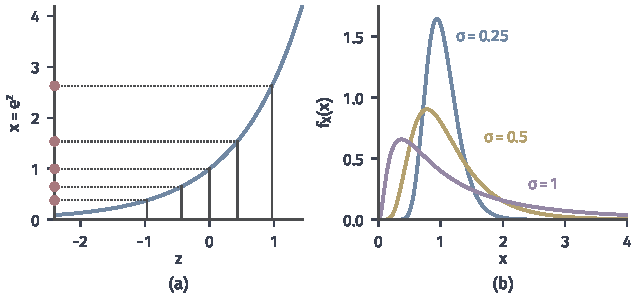
\includegraphics[width=108mm]{figures/07-probability/04-distribution-analysis/matplotlib/dfam-lognormal-map/figure.pdf}
  \caption{可逆非线性映射改变形状。(a)映射$x=\mathrm{e}^{z}$（蓝线）；横轴上深灰竖线把$\mathcal{N}(0,1)$分成六段等概率区间，分点经映射后在纵轴上的位置用红点标出，等概率区间的长度在$x$方向右侧拉长、左侧压缩。(b)$\mu=0$时$\sigma=0.25$（蓝）、$0.5$（黄）、$1$（紫）的对数正态密度，三者中位数都是$1$。}
  \label{fig:dfam-lognormal-map}
\end{BookInlineFigure}

换元公式在这里成立，靠的是映射同维、可逆、连续可微且导数不为零，第~\ref{chap:random-variable-transformations}章与\BookChapterRef{chap:pushforward-measures}{卷四第9章“推前测度”}都要求这些条件。条件破坏时，推前分布依然由式~\eqref{eq:dfam-pushforward}完全确定，只是不再有这样一个公式，甚至根本没有密度。下面两类映射就是这样。

\paragraph{把低维随机性放进高维空间}
取$Z\sim\operatorname{Unif}(0,1)$，参数$r>0$，令
\[
  \bm{X}_r=\bigl(r\cos(2\pi Z),\ r\sin(2\pi Z)\bigr).
\]
$\bm{X}_r$在半径为$r$的圆周上均匀分布，以概率$1$落在圆周上。圆周的平面面积为零，所以$\bm{X}_r$的分布不相对平面Lebesgue测度绝对连续，没有二维密度。参数$r$在这里控制的是支撑本身：不同的$r$给出的分布落在互不相交的圆周上。

这不是圆周的特殊性质。只要输入的维数低于输出，光滑映射的像就是零测集。

\begin{lemma}[低维像的零测性]
\label{lem:dfam-low-dim-image}
设$k<d$，$T:\mathbb{R}^{k}\to\mathbb{R}^{d}$连续可微。则$T(\mathbb{R}^{k})$是$\mathbb{R}^{d}$中的Borel集，且Lebesgue测度为零。因此对$\mathbb{R}^{k}$上任一概率测度$P_0$，$T_\#P_0$都没有相对$d$维Lebesgue测度的密度。
\end{lemma}

\begin{proof}
固定$R>0$，记$K_R=[-R,R]^{k}$。$K_R$是紧凸集，$DT$在$K_R$上连续，所以算子范数有上界$L$。由中值不等式，对$\bm{z},\bm{z}'\in K_R$，
\[
  \lVert T(\bm{z})-T(\bm{z}')\rVert_2\leq L\lVert\bm{z}-\bm{z}'\rVert_2 .
\]

把$K_R$等分成$m^{k}$个边长为$2R/m$的小立方体，每个的直径是$2R\sqrt{k}/m$。它的像落在半径为$2LR\sqrt{k}/m$的球内，从而落在边长为$4LR\sqrt{k}/m$的立方体内。把$m^{k}$块的体积加起来，
\[
  \lambda_d\bigl(T(K_R)\bigr)\leq m^{k}\Bigl(\frac{4LR\sqrt{k}}{m}\Bigr)^{d}=(4LR\sqrt{k})^{d}\,m^{k-d} .
\]
这里$T(K_R)$是紧集的连续像，仍是紧集，所以可测。由$k<d$，令$m\to\infty$，右边趋于零，所以$\lambda_d(T(K_R))=0$。

取$R=1,2,\dots$，$T(\mathbb{R}^{k})=\bigcup_RT(K_R)$是可数个紧集之并，是Borel集，测度为零。$T_\#P_0$在这个零测集上的质量是$P_0(\mathbb{R}^{k})=1$，所以它不相对$\lambda_d$绝对连续，没有密度。
\end{proof}

降维的方向相反时情况不同。$\bm{Z}\sim\mathcal{N}(\bm{0},\bm{I}_2)$，$X=Z_1+Z_2$把两个坐标并成一个，输出有密度，它是$\mathcal{N}(0,2)$；但这个密度不能用同维换元求得，要沿被合并的方向积分，即第~\ref{chap:random-variable-transformations}章的卷积。决定有没有密度的不是输入输出的维数谁大，而是映射是否把正的质量压进输出空间的零测集。线性映射$\bm{X}=\bm{A}\bm{Z}$中$\bm{A}$为奇异的$2\times2$矩阵时，像是一条直线，正是第~\ref{chap:multivariate-distributions}章退化高斯的情形。

\paragraph{离散化产生原子}
第三类映射把连续值归到有限或可数个格子里。取$Z\sim\mathcal{N}(0,1)$，位置参数$\mu$，令$X=\operatorname{round}(\mu+Z)$为最接近$\mu+Z$的整数（半整数处的取法不影响分布，因为那是零概率事件）。$X=k$当且仅当$k-\tfrac12\leq\mu+Z<k+\tfrac12$，所以
\begin{equation}
  \mathbb{P}(X=k)=\Phi\bigl(k+\tfrac12-\mu\bigr)-\Phi\bigl(k-\tfrac12-\mu\bigr),\qquad k\in\mathbb{Z}.
  \label{eq:dfam-rounding}
\end{equation}
连续的基础分布被推成一张概率表。取$\mu=0.3$，代入式~\eqref{eq:dfam-rounding}，
\[
  \mathbb{P}(X=-1)\approx0.176,\quad\mathbb{P}(X=0)\approx0.367,\quad\mathbb{P}(X=1)\approx0.306 .
\]

离散化也可以只作用在一部分取值上。令$X=\max(\mu+Z,0)$，负的读数都记成$0$。$\{X=0\}=\{Z\leq-\mu\}$，于是$\mathbb{P}(X=0)=\Phi(-\mu)$，$X$在$0$处有一个原子；在$(0,\infty)$上$X=\mu+Z$，有密度$\varphi(x-\mu)$。这个分布既不是概率表，也没有相对Lebesgue测度的密度。若取参考测度$\nu=\delta_0+\lambda_1$，它相对$\nu$的密度是
\[
  p(0)=\Phi(-\mu),\qquad p(x)=\varphi(x-\mu)\quad(x>0).
\]
$\mu=0.5$时原子的质量是$\Phi(-0.5)\approx0.309$。

\begin{BookInlineFigure}
  \centering
  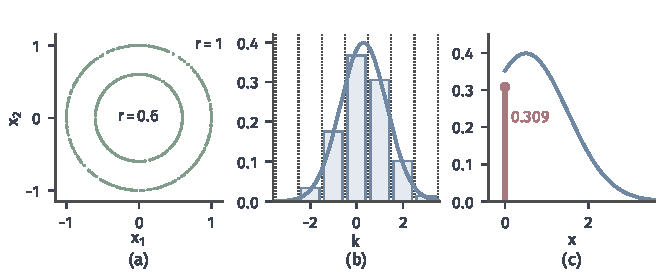
\includegraphics[width=112mm]{figures/07-probability/04-distribution-analysis/matplotlib/dfam-map-effects/figure.pdf}
  \caption{映射改变支撑与类型。(a)$Z\sim\operatorname{Unif}(0,1)$经$z\mapsto r(\cos2\pi z,\sin2\pi z)$得到的$400$个点（绿），$r=1$与$r=0.6$；分布全部落在圆周上，没有平面密度。(b)$\mu=0.3$时$\operatorname{round}(\mu+Z)$的概率表（浅蓝柱），蓝线是$\mu+Z$的密度，深灰竖线是格子边界$k\pm\tfrac12$。(c)$\max(\mu+Z,0)$，$\mu=0.5$：$(0,\infty)$上的密度（蓝线）与$0$处质量$0.309$的原子（红色竖线）。}
  \label{fig:dfam-map-effects}
\end{BookInlineFigure}

图~\ref{fig:dfam-map-effects}把三种结构放在一起。圆周上的分布支撑退化，取整得到概率表，截断得到原子与密度并存的混合类型。三者都是从有密度的基础分布出发、经过可测映射得到的，所以推前族的成员可以有任何类型；只有在同维可逆光滑的情形，才能放心地把它写成一个普通的密度模型。描述一般推前族时，应当用式~\eqref{eq:dfam-pushforward}和式~\eqref{eq:dfam-pushforward-expectation}，而不是先假定存在密度。


\section{混合分布}
\label{sec:dfam-mixtures}

一批零件来自两条生产线，一条偏大、一条偏小，混在一起测量，直方图上会出现两个峰。单个高斯分布无论怎样平移伸缩都只有一个峰，推前一个固定的高斯也不自然。更直接的描述是照着来源写：先随机决定零件来自哪条线，再按那条线的规律产生尺寸。这样得到的分布族，参数分成两类：选择成分的规律，以及各成分自己的参数。

\subsection{有限混合}
\label{sec:dfam-finite-mixture}

设$P_1,\dots,P_m$是$\mathcal{X}$上的概率测度，$\bm{w}=(w_1,\dots,w_m)$是一张概率表。先抽成分指标$K$，$\mathbb{P}(K=k)=w_k$；再在$K=k$的条件下让$X\sim P_k$。由第~\ref{chap:conditional-distributions}章的全概率公式，
\[
  \begin{aligned}
    \mathbb{P}(X\in B)&=\sum_{k=1}^{m}\mathbb{P}(K=k)\,\mathbb{P}(X\in B\mid K=k)\\
    &=\sum_{k=1}^{m}w_kP_k(B).
  \end{aligned}
\]

\begin{definition}[有限混合]
\label{def:dfam-finite-mixture}
设$\bm{w}\in\Delta_{m-1}$，$P_1,\dots,P_m\in\mathcal{P}(\mathcal{X})$。概率测度
\begin{equation}
  P=\sum_{k=1}^{m}w_kP_k
  \label{eq:dfam-finite-mixture}
\end{equation}
称为成分$P_1,\dots,P_m$以\term{混合权重}（mixture weights）$\bm{w}$构成的\term{有限混合}（finite mixture）。若各成分取自一个参数化族，$P_k=Q_{\bm{\eta}_k}$，则混合族的参数是$(\bm{w},\bm{\eta}_1,\dots,\bm{\eta}_m)$。
\end{definition}

式~\eqref{eq:dfam-finite-mixture}是概率的加权平均，对每个事件逐一成立。所以分布函数、密度（若各成分相对同一个$\nu$有密度$p_k$）和有限的期望都按同样的权重相加：
\[
  F=\sum_kw_kF_k,\qquad p=\sum_kw_kp_k,\qquad\mathbb{E}_P[g]=\sum_kw_k\,\mathbb{E}_{P_k}[g].
\]
分位数不在其列。分位数函数是分布函数的广义逆，逆运算与加权平均不能交换，混合的中位数一般不等于各成分中位数的加权平均。

\paragraph{均值与方差}
设第$k$个成分的均值与方差为$m_k$、$s_k^{2}$，记$\bar{m}=\sum_kw_km_k$。由上式，$\mathbb{E}[X]=\bar{m}$。方差由全方差公式（第~\ref{chap:conditional-expectation}章）给出，其中两个条件量是
\[
  \mathbb{E}[X\mid K]=m_K,\qquad\operatorname{Var}(X\mid K)=s_K^{2},
\]
代入得到
\begin{equation}
  \operatorname{Var}(X)=\sum_{k}w_ks_k^{2}+\sum_kw_k(m_k-\bar{m})^{2}.
  \label{eq:dfam-mixture-variance}
\end{equation}
第一项是成分内部的平均波动，第二项是成分中心之间的分散。若把各成分看成放在$m_k$处的质量块，第二项正是这组质量块绕总重心的转动惯量。

\paragraph{两个高斯成分}
取等权的两个成分$\mathcal{N}(-a,1)$与$\mathcal{N}(a,1)$，$a>0$，混合密度是
\[
  f_a(x)=\tfrac12\varphi(x+a)+\tfrac12\varphi(x-a).
\]
由式~\eqref{eq:dfam-mixture-variance}，均值是$0$，方差是$1+a^{2}$。取$a=1.5$，方差是$3.25$，比每个成分的方差$1$大得多，多出的$2.25$全部来自两个中心的分离。

$f_a$关于$0$对称，所以$f_a'(0)=0$。要判断$0$处是峰还是谷，看二阶导数。$\varphi'(z)=-z\varphi(z)$，再求一次导，
\[
  \varphi''(z)=(z^{2}-1)\varphi(z).
\]
代入$f_a$，两项在$x=0$处相等，得到
\begin{equation}
  f_a''(0)=(a^{2}-1)\,\varphi(a).
  \label{eq:dfam-mixture-curvature}
\end{equation}

$a<1$时$f_a''(0)<0$，中心是局部极大；$a>1$时$f_a''(0)>0$，中心变成局部极小。后一种情形下$f_a$在$0$处是谷，又在$\pm\infty$处趋于零，所以两侧各有一个峰，密度至少有两个峰。$a=1$是转折点，两个成分中心相距$2$，恰为成分标准差的两倍。图~\ref{fig:dfam-mixture-separation}画出$a=0.5,1,1.5,2$的情形。

\begin{BookInlineFigure}
  \centering
  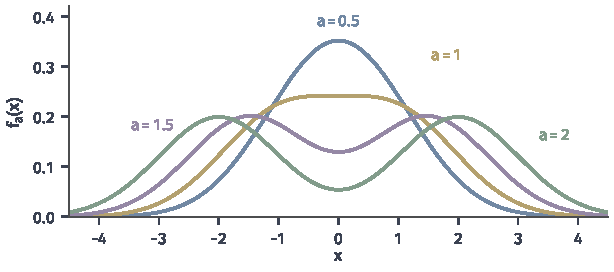
\includegraphics[width=104mm]{figures/07-probability/04-distribution-analysis/matplotlib/dfam-mixture-separation/figure.pdf}
  \caption{等权混合$\frac12\mathcal{N}(-a,1)+\frac12\mathcal{N}(a,1)$的密度，$a=0.5$（蓝）、$1$（黄）、$1.5$（紫）、$2$（绿）。$a=1$时中心处的二阶导数为零，顶部最平；$a>1$时中心是谷，出现两个峰。}
  \label{fig:dfam-mixture-separation}
\end{BookInlineFigure}

单个高斯分布的密度从中心向两侧单调下降，只有一个峰；$\mathcal{N}(0,1)$生成的位置尺度族中所有成员都是如此。两个高斯的混合却能有两个峰。这是混合族比它的成分族多出来的形状。

\paragraph{只改权重与改变成分}
混合族的两类参数作用不同。固定成分只改权重，密度$p=\sum_kw_kp_k$对$\bm{w}$是线性的：权重把质量在几块固定的形状之间重新分配，峰的位置大体不动，峰的高低此消彼长。全体权重给出的分布构成一个凸集，第~\ref{sec:dfam-candidates}节三角形中的线段就是两个概率表的全部混合。

改变成分参数则改变形状本身，密度对它们是非线性的。图~\ref{fig:dfam-mixture-weights-params}(a)固定$a=1.5$，把第二个成分的权重从$0.5$增到$0.9$，右峰升高、左峰缩成肩部；(b)固定等权，把第二个成分的标准差缩小到$0.5$、中心移到$2$，右峰变得又窄又高，左峰的形状不变。

\begin{BookInlineFigure}
  \centering
  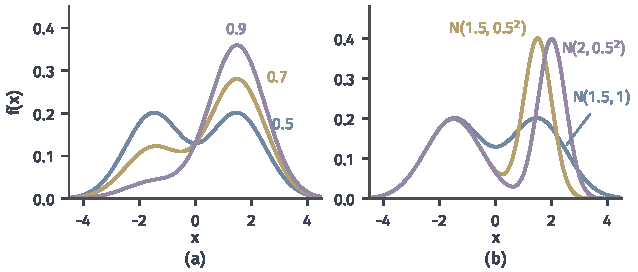
\includegraphics[width=108mm]{figures/07-probability/04-distribution-analysis/matplotlib/dfam-mixture-weights-params/figure.pdf}
  \caption{混合族中两类参数的作用。(a)成分固定为$\mathcal{N}(-1.5,1)$与$\mathcal{N}(1.5,1)$，第二个成分的权重为$0.5$（蓝）、$0.7$（黄）、$0.9$（紫）。(b)等权，第二个成分为$\mathcal{N}(1.5,1)$（蓝）、$\mathcal{N}(1.5,0.5^{2})$（黄）、$\mathcal{N}(2,0.5^{2})$（紫）；第一个成分始终是$\mathcal{N}(-1.5,1)$。}
  \label{fig:dfam-mixture-weights-params}
\end{BookInlineFigure}

\paragraph{混合不是取值的平均}
“按权重$\tfrac12,\tfrac12$组合两个随机量”有两种截然不同的意思。设$Y_1\sim\mathcal{N}(-1.5,1)$与$Y_2\sim\mathcal{N}(1.5,1)$独立。混合是以概率$\tfrac12$报告$Y_1$、以概率$\tfrac12$报告$Y_2$，分布是$f_{1.5}$，方差$3.25$。取值的平均$\tfrac12Y_1+\tfrac12Y_2$则是两个独立高斯的线性组合，由第~\ref{chap:multivariate-distributions}章，它服从
\[
  \mathcal{N}\bigl(0,\ \tfrac14+\tfrac14\bigr)=\mathcal{N}(0,0.5).
\]
它只有一个峰，方差只有$0.5$。

两者的差别在于加权的对象。混合对概率加权，每次只取一个成分的值，两个峰都保留下来；取值平均对随机变量加权，每次都把两个值折中，正负偏离互相抵消。图~\ref{fig:dfam-mix-vs-sum}并排画出两者。

\begin{BookInlineFigure}
  \centering
  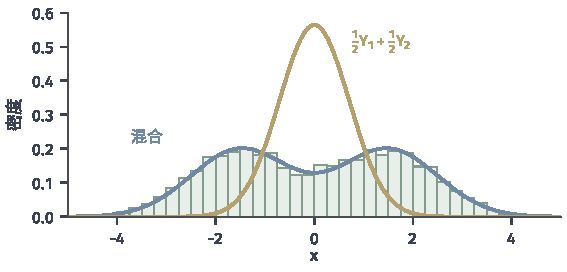
\includegraphics[width=96mm]{figures/07-probability/04-distribution-analysis/matplotlib/dfam-mix-vs-sum/figure.pdf}
  \caption{同一对成分$\mathcal{N}(-1.5,1)$、$\mathcal{N}(1.5,1)$的两种“等权组合”。蓝线是混合$\frac12\mathcal{N}(-1.5,1)+\frac12\mathcal{N}(1.5,1)$，方差$3.25$；黄线是独立变量的平均$\frac12Y_1+\frac12Y_2\sim\mathcal{N}(0,0.5)$。绿色直方图是混合的$5000$个模拟样本（种子$716$）。}
  \label{fig:dfam-mix-vs-sum}
\end{BookInlineFigure}

\subsection{连续混合}
\label{sec:dfam-continuous-mixture}

有限混合的成分指标只取有限个值。若影响结果的隐藏因素是连续的，例如每个零件的加工精度都略有不同，就要让成分由一个连续变量$S$索引。给定$S=s$时，$X$的条件分布是$K(s,\cdot)$；$S$本身服从分布$M$。

\begin{definition}[一般混合]
\label{def:dfam-general-mixture}
设$(\mathcal{S},\mathcal{F}_{\mathcal{S}})$上有概率测度$M$，$K$是从$\mathcal{S}$到$\mathcal{X}$的概率核。概率测度
\begin{equation}
  P(B)=\int_{\mathcal{S}}K(s,B)\,M(\mathrm{d}s),\qquad B\in\mathcal{F}_{\mathcal{X}},
  \label{eq:dfam-general-mixture}
\end{equation}
称为核$K$以\term{混合测度}（mixing measure）$M$构成的混合。$M$不是离散分布时，常称为\term{连续混合}（continuous mixture）。
\end{definition}

$P$确实是概率测度：$K(s,\mathcal{X})=1$给出$P(\mathcal{X})=1$；对互不相交的$B_1,B_2,\dots$，$K(s,\cdot)$可数可加，再由单调收敛定理交换求和与积分，得到$P$可数可加。式~\eqref{eq:dfam-general-mixture}正是第~\ref{chap:conditional-distributions}章由边缘分布与条件分布恢复$X$的边缘分布的公式，这里把它反过来用作构造。取$M=\sum_kw_k\delta_k$，积分退回求和，得到式~\eqref{eq:dfam-finite-mixture}。

若每个$K(s,\cdot)$相对同一个$\nu$有密度$k(x\mid s)$，且$k$对$(s,x)$联合可测，则由Tonelli定理交换积分次序，
\[
  P(B)=\int_{\mathcal{S}}\int_Bk(x\mid s)\,\nu(\mathrm{d}x)\,M(\mathrm{d}s)=\int_B\Bigl(\int_{\mathcal{S}}k(x\mid s)\,M(\mathrm{d}s)\Bigr)\nu(\mathrm{d}x).
\]
所以混合的密度是条件密度按$M$的平均：
\begin{equation}
  p(x)=\int_{\mathcal{S}}k(x\mid s)\,M(\mathrm{d}s).
  \label{eq:dfam-mixture-density}
\end{equation}

\paragraph{正态尺度混合}
最常用的连续混合是第~\ref{chap:multivariate-distributions}章的正态尺度混合：$W\geq0$与$Z\sim\mathcal{N}(0,1)$独立，$X=\sqrt{W}Z$。给定$W=w$，$X\sim\mathcal{N}(0,w)$，混合测度是$W$的分布。那一章用它构造了t分布与Laplace分布；这里关心的是，不管$W$怎样分布，混合都带来什么共同的形状。

\begin{theorem}[尺度混合使峰度不小于三]
\label{thm:dfam-scale-mixture-kurtosis}
设$W\geq0$，$\mathbb{E}[W^{2}]<\infty$，$\mathbb{P}(W>0)>0$，$Z\sim\mathcal{N}(0,1)$与$W$独立，$X=\sqrt{W}Z$。则$X$的峰度
\begin{equation}
  \kappa(X)=\frac{\mathbb{E}[X^{4}]}{(\mathbb{E}[X^{2}])^{2}}=\frac{3\,\mathbb{E}[W^{2}]}{(\mathbb{E}[W])^{2}}\geq3 ,
  \label{eq:dfam-scale-kurtosis}
\end{equation}
等号成立当且仅当$W$几乎必然为常数。
\end{theorem}

\begin{proof}
$X$的均值是$\mathbb{E}[\sqrt{W}]\,\mathbb{E}[Z]=0$。由独立性与$\mathbb{E}[Z^{2}]=1$、$\mathbb{E}[Z^{4}]=3$，
\[
  \mathbb{E}[X^{2}]=\mathbb{E}[W]\,\mathbb{E}[Z^{2}]=\mathbb{E}[W],\qquad\mathbb{E}[X^{4}]=\mathbb{E}[W^{2}]\,\mathbb{E}[Z^{4}]=3\,\mathbb{E}[W^{2}].
\]
由$\mathbb{P}(W>0)>0$，$\mathbb{E}[W]>0$，比值有意义。由方差非负，
\[
  \mathbb{E}[W^{2}]-(\mathbb{E}[W])^{2}=\operatorname{Var}(W)\geq0 ,
\]
所以$\kappa(X)\geq3$；等号成立当且仅当$\operatorname{Var}(W)=0$，即$W$几乎必然等于常数。
\end{proof}

高斯分布的峰度恰好是$3$。定理说，只要尺度真的随机，混合的峰度就严格大于$3$：大的$W$贡献远处的值，小的$W$贡献贴近$0$的值，结果比同方差的高斯分布中间更尖、尾部更厚。例如$W$以各$\tfrac12$的概率取$0.5$和$1.5$，这是两成分的有限混合，
\[
  \mathbb{E}[W]=1,\qquad\mathbb{E}[W^{2}]=\tfrac12(0.25+2.25)=1.25,\qquad\kappa(X)=3.75 .
\]
取$W\sim\operatorname{Exp}(1)$，$\mathbb{E}[W]=1$，$\mathbb{E}[W^{2}]=2$，由式~\eqref{eq:dfam-scale-kurtosis}得$\kappa(X)=6$；第~\ref{chap:multivariate-distributions}章算出这时$X$服从$\operatorname{Laplace}(0,1/\sqrt2)$，其峰度正是$6$。

\paragraph{共同尺度带来的依赖}
在多元情形，同一个$W$乘到所有分量上。设$\bm{Z}\sim\mathcal{N}(\bm{0},\bm{I}_2)$与$W$独立，$\bm{X}=\sqrt{W}\bm{Z}$，$\mathbb{E}[W^{2}]<\infty$。由独立性，
\[
  \operatorname{Cov}(\bm{X})=\mathbb{E}[W]\,\bm{I}_2 ,
\]
两个分量不相关。但它们不独立：
\[
  \mathbb{E}[X_1^{2}X_2^{2}]=\mathbb{E}[W^{2}]\,\mathbb{E}[Z_1^{2}]\,\mathbb{E}[Z_2^{2}]=\mathbb{E}[W^{2}],
\]
而两个边缘二阶矩的乘积是
\[
  \mathbb{E}[X_1^{2}]\,\mathbb{E}[X_2^{2}]=(\mathbb{E}[W])^{2}.
\]
若$W$不是常数，两者不等，$X_1^{2}$与$X_2^{2}$正相关，所以$X_1,X_2$不独立。$W\sim\operatorname{Exp}(1)$时
\[
  \operatorname{Cov}(X_1^{2},X_2^{2})=\mathbb{E}[W^{2}]-(\mathbb{E}[W])^{2}=1 .
\]

直观上，$W$大的那一次，两个分量同时被放大；$W$小的那一次，两个分量同时贴近原点。图~\ref{fig:dfam-scale-mixture}(b)中，离原点较远的点（红）均匀地散在各个方向上，包括对角方向，说明两个分量常常一起取大值；(c)让每个分量各用一个独立的$W_i$，边缘分布与(b)完全相同，远处的点却集中在两条坐标轴附近：一个分量很大时，另一个分量通常仍然不大。只看边缘分布或协方差，分不出这两种模型。

\begin{BookInlineFigure}
  \centering
  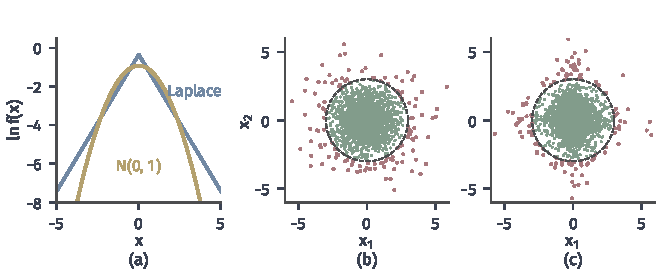
\includegraphics[width=112mm]{figures/07-probability/04-distribution-analysis/matplotlib/dfam-scale-mixture/figure.pdf}
  \caption{正态尺度混合，$W\sim\operatorname{Exp}(1)$。(a)一元密度的对数：$X=\sqrt{W}Z$即$\operatorname{Laplace}(0,1/\sqrt2)$（蓝），与同方差的$\mathcal{N}(0,1)$（黄）；混合的中心更尖、尾部按直线而非抛物线下降。(b)共同尺度$\sqrt{W}(Z_1,Z_2)$的$3000$个样本。(c)独立尺度$(\sqrt{W_1}Z_1,\sqrt{W_2}Z_2)$的$3000$个样本。(b)(c)中深灰虚线是半径$3$的圆，圆外的点标红；两图的边缘分布相同，协方差都是$\bm{I}_2$；模拟种子$716$。}
  \label{fig:dfam-scale-mixture}
\end{BookInlineFigure}

\paragraph{计数的混合}
连续混合同样适用于离散结果。设给定$\Lambda=\lambda$时$X\sim\operatorname{Poisson}(\lambda)$，而强度$\Lambda\sim\operatorname{Gamma}(\alpha,\beta)$。由式~\eqref{eq:dfam-mixture-density}，以计数测度为参考，
\[
  \mathbb{P}(X=k)=\int_0^\infty\mathrm{e}^{-\lambda}\frac{\lambda^{k}}{k!}\cdot\frac{\beta^{\alpha}\lambda^{\alpha-1}\mathrm{e}^{-\beta\lambda}}{\Gamma(\alpha)}\,\mathrm{d}\lambda .
\]

把$\lambda$的幂与指数合并，剩下的积分是一个Gamma积分，
\[
  \int_0^\infty\lambda^{k+\alpha-1}\mathrm{e}^{-(1+\beta)\lambda}\,\mathrm{d}\lambda=\frac{\Gamma(k+\alpha)}{(1+\beta)^{k+\alpha}} .
\]
代回得到
\begin{equation}
  \mathbb{P}(X=k)=\frac{\Gamma(k+\alpha)}{k!\,\Gamma(\alpha)}\Bigl(\frac{\beta}{1+\beta}\Bigr)^{\alpha}\Bigl(\frac{1}{1+\beta}\Bigr)^{k},\qquad k=0,1,\dots
  \label{eq:dfam-negative-binomial}
\end{equation}
这是\term{负二项分布}（negative binomial distribution）。

取$\alpha=2$、$\beta=1$，式~\eqref{eq:dfam-negative-binomial}化为$\mathbb{P}(X=k)=(k+1)/2^{k+2}$，前几项是
\[
  p_0=\tfrac14,\quad p_1=\tfrac14,\quad p_2=\tfrac{3}{16},\quad p_3=\tfrac18 .
\]
均值由全期望公式得$\mathbb{E}[\Lambda]=\alpha/\beta=2$，与$\operatorname{Poisson}(2)$相同。方差由全方差公式得
\[
  \operatorname{Var}(X)=\mathbb{E}[\Lambda]+\operatorname{Var}(\Lambda)=\frac{\alpha}{\beta}+\frac{\alpha}{\beta^{2}}=4 ,
\]
是$\operatorname{Poisson}(2)$方差的两倍。强度的随机性使$0$和大计数都更常见：$p_0=0.25$，而$\operatorname{Poisson}(2)$在$0$处只有$\mathrm{e}^{-2}\approx0.135$，见图~\ref{fig:dfam-poisson-gamma}。

\begin{BookInlineFigure}
  \centering
  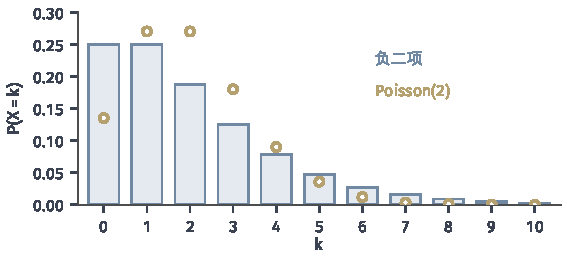
\includegraphics[width=96mm]{figures/07-probability/04-distribution-analysis/matplotlib/dfam-poisson-gamma/figure.pdf}
  \caption{计数的连续混合。浅蓝柱是$\operatorname{Poisson}(\Lambda)$、$\Lambda\sim\operatorname{Gamma}(2,1)$的混合，即负二项分布$(k+1)/2^{k+2}$；黄色空心点是同均值的$\operatorname{Poisson}(2)$。两者均值都是$2$，方差分别为$4$与$2$。}
  \label{fig:dfam-poisson-gamma}
\end{BookInlineFigure}

\paragraph{改变混合测度与改变核}
连续混合族有两个可以变动的部分。固定核$K(w,\cdot)=\mathcal{N}(0,w)$，让混合测度$M$取遍$(0,\infty)$上全体概率测度，得到全体正态尺度混合。这个族是凸的，包含所有t分布与上面的Laplace分布，远比任何有限维族大；但它的成员都关于$0$对称，由定理~\ref{thm:dfam-scale-mixture-kurtosis}，四阶矩有限的成员峰度都不小于$3$。

所以改变$M$无论怎样都造不出偏斜的分布，也造不出比高斯更“平”的分布。$\operatorname{Unif}(-\sqrt3,\sqrt3)$的方差为$1$，峰度为$1.8$，它就不是任何正态尺度混合。要得到这些形状，必须换掉核：例如把$\mathcal{N}(0,w)$换成$\mathcal{N}(s,1)$，让混合测度作用在位置上，或者像Poisson–Gamma那样换成离散的核。混合测度决定成分怎样搭配，核决定可以搭配的成分是什么形状。

\subsection{混合表示的非唯一性}
\label{sec:dfam-mixture-nonuniqueness}

混合族的参数比分布多出很多冗余。第~\ref{sec:dfam-identifiability}节已经看到标签置换；这里把各种冗余列清楚，再说明成分互相重叠并不是冗余。

\paragraph{冗余从哪里来}
考虑等方差的两成分高斯混合
\[
  P_{(w,\mu_1,\mu_2)}=w\,\mathcal{N}(\mu_1,1)+(1-w)\,\mathcal{N}(\mu_2,1),\qquad 0\leq w\leq1 .
\]
第一种冗余是标签置换：$(w,\mu_1,\mu_2)$与$(1-w,\mu_2,\mu_1)$给出同一个分布。它把参数成对地粘在一起，每个真正的两成分分布恰好对应两组参数。

第二种冗余来自重复成分。$\mu_1=\mu_2=\mu$时，两个成分相同，
\[
  w\,\mathcal{N}(\mu,1)+(1-w)\,\mathcal{N}(\mu,1)=\mathcal{N}(\mu,1)
\]
对每个$w\in[0,1]$成立，权重完全看不见。第三种冗余来自零权重：$w=0$时，$\mu_1$不出现在分布中，可以取任意值。

以$\mathcal{N}(0,1)$为例，它的全部表示是
\[
  \{w\in[0,1],\ \mu_1=\mu_2=0\}\cup\{w=0,\ \mu_2=0\}\cup\{w=1,\ \mu_1=0\}.
\]
这是参数空间中的三条线段（其中两条是整条直线），不再是孤立的点。图~\ref{fig:dfam-mixture-fibers}(a)在$\mu_2=0$的截面上画出其中两条：$\mu_1=0$的竖线与$w=0$的横线交成一个十字。

\begin{BookInlineFigure}
  \centering
  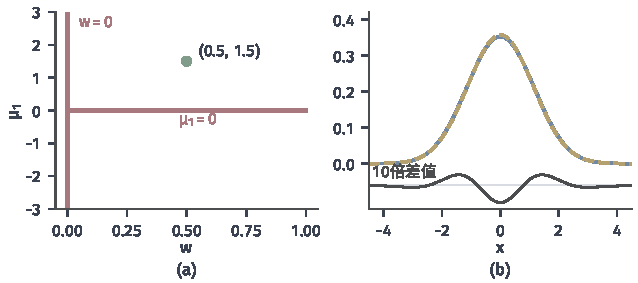
\includegraphics[width=108mm]{figures/07-probability/04-distribution-analysis/matplotlib/dfam-mixture-fibers/figure.pdf}
  \caption{混合表示的冗余与重叠。(a)$\mu_2=0$的截面$(w,\mu_1)$中，给出$\mathcal{N}(0,1)$的参数（红线）：$\mu_1=0$时任何$w$都可以，$w=0$时任何$\mu_1$都可以；绿点是$(0.5,1.5)$，代表一个真正的两成分混合，它在这个截面上只出现一次。(b)重叠很大的混合$\frac12\mathcal{N}(-0.5,1)+\frac12\mathcal{N}(0.5,1)$（蓝）与同均值、同方差的$\mathcal{N}(0,1.25)$（黄）；下方深灰线是两者密度之差，放大$10$倍。}
  \label{fig:dfam-mixture-fibers}
\end{BookInlineFigure}

\paragraph{重叠不等于不可辨识}
成分互相重叠是另一回事。$\tfrac12\mathcal{N}(-0.5,1)+\tfrac12\mathcal{N}(0.5,1)$的两个成分大部分重合，混合只有一个峰，看上去几乎就是一个高斯：图~\ref{fig:dfam-mixture-fibers}(b)中它与同均值同方差的$\mathcal{N}(0,1.25)$的密度之差最大不到$0.005$，约为峰高的$1.4\%$。但两者是不同的分布，而且下面的定理说明，这个混合的参数除了标签置换外是唯一确定的。

记$\varphi_\sigma(x)=\varphi(x/\sigma)/\sigma$为$\mathcal{N}(0,\sigma^{2})$的密度。证明要用到一个关于指数函数的事实。

\begin{lemma}[不同指数的指数函数线性无关]
\label{lem:dfam-exp-independent}
设$\nu_1>\nu_2>\cdots>\nu_r$为实数，$c_1,\dots,c_r$为实数。若对一切$t\in\mathbb{R}$有$\sum_{j=1}^{r}c_j\mathrm{e}^{\nu_jt}=0$，则$c_1=\cdots=c_r=0$。
\end{lemma}

\begin{proof}
两边乘以$\mathrm{e}^{-\nu_1t}$，得
\[
  c_1+\sum_{j=2}^{r}c_j\mathrm{e}^{(\nu_j-\nu_1)t}=0 .
\]
各$\nu_j-\nu_1<0$，令$t\to+\infty$，求和项趋于零，所以$c_1=0$。对剩下的$r-1$项重复这一步，依次得到$c_2=\cdots=c_r=0$。
\end{proof}

\begin{theorem}[已知方差的高斯位置混合可辨识]
\label{thm:dfam-gaussian-mixture-identifiable}
固定$\sigma>0$。设$\mu_1,\dots,\mu_m$互不相同，$\mu'_1,\dots,\mu'_{m'}$互不相同，权重$w_k>0$、$w'_l>0$且各自和为$1$。若
\begin{equation}
  \sum_{k=1}^{m}w_k\,\mathcal{N}(\mu_k,\sigma^{2})=\sum_{l=1}^{m'}w'_l\,\mathcal{N}(\mu'_l,\sigma^{2}),
  \label{eq:dfam-mixture-equal}
\end{equation}
则$m=m'$，且存在$\{1,\dots,m\}$的置换$\pi$，使$\mu'_{\pi(k)}=\mu_k$、$w'_{\pi(k)}=w_k$。
\end{theorem}

\begin{proof}
两边是同一个分布，所以对一切$t$，$\mathrm{e}^{tX}$在两边的期望相同。$\mathcal{N}(\mu,\sigma^{2})$的矩母函数是$\mathrm{e}^{\mu t+\sigma^{2}t^{2}/2}$，有限混合的矩母函数是成分矩母函数的加权和，于是
\[
  \mathrm{e}^{\sigma^{2}t^{2}/2}\sum_{k}w_k\mathrm{e}^{\mu_kt}=\mathrm{e}^{\sigma^{2}t^{2}/2}\sum_{l}w'_l\mathrm{e}^{\mu'_lt},\qquad t\in\mathbb{R}.
\]
约去公共因子$\mathrm{e}^{\sigma^{2}t^{2}/2}>0$，移项，
\[
  \sum_{k}w_k\mathrm{e}^{\mu_kt}-\sum_lw'_l\mathrm{e}^{\mu'_lt}=0,\qquad t\in\mathbb{R}.
\]

把两组位置合在一起，按不同的值合并同类项。对每个出现过的值$\nu$，它的系数是“$\nu$在左边的权重”减去“$\nu$在右边的权重”，在一边没有出现时那一边记为零。由引理~\ref{lem:dfam-exp-independent}，每个系数都为零。若某个$\mu_k$不在右边出现，它的系数就是$w_k>0$，矛盾；所以每个$\mu_k$都等于某个$\mu'_l$，且权重相同。对右边同样论证，两组位置作为集合相同，于是$m=m'$，对应的权重相等。
\end{proof}

定理的条件都有作用。位置互不相同、权重为正，排除了重复成分与零权重两种冗余；结论中的置换$\pi$就是标签置换，它无法消除。方差$\sigma^{2}$固定已知也很关键：它让公共因子$\mathrm{e}^{\sigma^{2}t^{2}/2}$可以约去。

\paragraph{成分族决定能否识别}
可辨识的条件要按所用的成分族逐一核对，不能从高斯推到别的族。Bernoulli成分是最极端的反例：对任意$w,a,b\in[0,1]$，
\[
  w\operatorname{Bern}(a)+(1-w)\operatorname{Bern}(b)=\operatorname{Bern}\bigl(wa+(1-w)b\bigr).
\]
无论成分怎样分开，混合仍是一个Bernoulli分布，只有一个数$wa+(1-w)b$可见，三个参数中有两个完全无法确定。均匀成分也有类似现象：
\[
  \tfrac12\operatorname{Unif}(0,1)+\tfrac12\operatorname{Unif}(1,2)=\operatorname{Unif}(0,2),
\]
一个两成分表示与一个单成分表示给出同一个分布。

这两个例子与高斯的差别不在于成分是否重叠，均匀的例子中两个成分根本不重叠。差别在于成分族本身在混合下是否“封闭”：Bernoulli族的混合仍在Bernoulli族里，均匀分布可以切成更小的均匀分布再拼回去。高斯成分做不到这一点，定理~\ref{thm:dfam-gaussian-mixture-identifiable}的证明正是利用了矩母函数中不同的指数无法互相抵消。


\section{Copula表示}
\label{sec:dfam-copulas}

两台设备的寿命$X_1,X_2$都服从$\operatorname{Exp}(1)$。只凭这一点，还说不出两台设备都在一年内损坏的概率：若两台互不影响，它是$(1-\mathrm{e}^{-1})^{2}\approx0.400$；若两台总是同时损坏，它是$1-\mathrm{e}^{-1}\approx0.632$。边缘分布相同，联合分布却可以很不一样。我们想把联合分布中“边缘以外的部分”单独拿出来，作为一个可以与任何边缘搭配的对象。

\subsection{边缘与依赖的分离}
\label{sec:dfam-copula-separation}

把每个分量都换成均匀分布的刻度，各分量自己的规律就被抹掉了，剩下的只有它们怎样一起变化。

\begin{definition}[Copula]
\label{def:dfam-copula}
设随机向量$\bm{U}=(U_1,\dots,U_d)$的每个分量都服从$\operatorname{Unif}(0,1)$。$\bm{U}$的联合分布函数在$[0,1]^{d}$上的限制
\begin{equation}
  C(u_1,\dots,u_d)=\mathbb{P}(U_1\leq u_1,\dots,U_d\leq u_d)
  \label{eq:dfam-copula}
\end{equation}
称为一个Copula。
\end{definition}

Copula就是边缘全为均匀分布的联合分布函数。最简单的三个例子都在$d=2$时看。$U_1,U_2$独立时，
\[
  \Pi(u,v)=uv ,
\]
称为\term{乘积Copula}（product copula）。取一个均匀变量$U$，令$U_1=U_2=U$，两个分量完全同向变化，
\[
  M(u,v)=\mathbb{P}(U\leq u,\ U\leq v)=\min(u,v).
\]
令$U_1=U$、$U_2=1-U$，两个分量完全反向变化，
\[
  W(u,v)=\mathbb{P}(U\leq u,\ 1-U\leq v)=\max(u+v-1,\,0).
\]
另一个常用的例子来自高斯向量。设$(G_1,G_2)$是标准化的二元高斯向量，相关系数为$\rho$。$\Phi$连续且严格增，所以对$0<u<1$，
\[
  \mathbb{P}\bigl(\Phi(G_i)\leq u\bigr)=\mathbb{P}\bigl(G_i\leq\Phi^{-1}(u)\bigr)=u ,
\]
$(\Phi(G_1),\Phi(G_2))$的边缘都是均匀的，它的联合分布函数$C_\rho$称为\term{高斯Copula}（Gaussian copula）。

\paragraph{用Copula拼出联合分布}
给定一个Copula和任意一组边缘分布，可以拼出联合分布。办法是把均匀变量按各自的分位数函数送到目标刻度上，这正是第~\ref{chap:random-variables}章由$\operatorname{Unif}(0,1)$生成任意分布的办法，只是现在$d$个均匀变量带着依赖一起被送过去。这个构造与它的逆向结论合称\term{Sklar定理}（Sklar's theorem）。

\begin{theorem}[Sklar定理]
\label{thm:dfam-sklar}
\begin{enumerate}
  \item 设$C$是$d$元Copula，$F_1,\dots,F_d$是一元分布函数。则
  \begin{equation}
    F(x_1,\dots,x_d)=C\bigl(F_1(x_1),\dots,F_d(x_d)\bigr)
    \label{eq:dfam-sklar}
  \end{equation}
  是一个$d$元联合分布函数，其第$i$个边缘分布函数为$F_i$。
  \item 反之，设$F$是$d$元联合分布函数，边缘分布函数为$F_1,\dots,F_d$。则存在Copula $C$使式~\eqref{eq:dfam-sklar}成立，并且$C$在$\operatorname{Ran}F_1\times\cdots\times\operatorname{Ran}F_d$上由$F$唯一确定，其中$\operatorname{Ran}F_i$是$F_i$的值域。
\end{enumerate}
\end{theorem}

\begin{proof}[第一部分的证明]
设$\bm{U}$的联合分布函数为$C$，$Q_i$为$F_i$的分位数函数，令$X_i=Q_i(U_i)$。每个$U_i$均匀，所以$\mathbb{P}(U_i\in\{0,1\})=0$，下面可以只考虑$U_i\in(0,1)$。第~\ref{chap:random-variables}章的引理给出：对$u\in(0,1)$，
\[
  Q_i(u)\leq x\iff u\leq F_i(x).
\]
于是事件$\{X_i\leq x_i\}$与$\{U_i\leq F_i(x_i)\}$几乎必然相同，对$i=1,\dots,d$同时成立，所以
\[
  \begin{aligned}
    \mathbb{P}(X_1\leq x_1,\dots,X_d\leq x_d)&=\mathbb{P}\bigl(U_1\leq F_1(x_1),\dots,U_d\leq F_d(x_d)\bigr)\\
    &=C\bigl(F_1(x_1),\dots,F_d(x_d)\bigr).
  \end{aligned}
\]
左边是随机向量$(X_1,\dots,X_d)$的联合分布函数，所以式~\eqref{eq:dfam-sklar}是联合分布函数。由同一章的定理，$X_i=Q_i(U_i)$的分布函数是$F_i$，这就是第$i$个边缘。
\end{proof}

第二部分的证明要把一般的$\bm{X}$送回均匀刻度，边缘有没有原子会使做法和结论都不同，留到下一小节。

第一部分已经说明了分离的含义：边缘$F_1,\dots,F_d$与Copula $C$可以独立地选。同一组边缘配上不同的$C$，得到不同的联合分布；同一个$C$配上不同的边缘，依赖的“样式”保持不变。

\paragraph{两台设备}
回到本节开头的两台设备，$F_1=F_2$为$\operatorname{Exp}(1)$的分布函数，$F_1(1)=1-\mathrm{e}^{-1}\approx0.632$。由式~\eqref{eq:dfam-sklar}，两台都在一年内损坏的概率是$C(0.632,0.632)$。代入三个Copula，
\[
  \Pi:\ 0.632^{2}\approx0.400,\qquad M:\ 0.632,\qquad W:\ 2\times0.632-1\approx0.264 .
\]
高斯Copula取$\rho=0.7$时，这个概率是$\mathbb{P}(G_1\leq z,G_2\leq z)$，其中$z=\Phi^{-1}(0.632)\approx0.337$，数值积分得约$0.513$，介于独立与完全同向之间。

图~\ref{fig:dfam-copula-samples}上排是三个Copula的样本，都在单位正方形中；下排把同一批样本用$Q(u)=-\ln(1-u)$送到$\operatorname{Exp}(1)$的刻度上。下排三幅图的两个边缘完全相同，点的排列却各不相同：独立时散成一片，高斯Copula时沿对角线聚集，完全同向时全部落在对角线上。

\begin{BookInlineFigure}
  \centering
  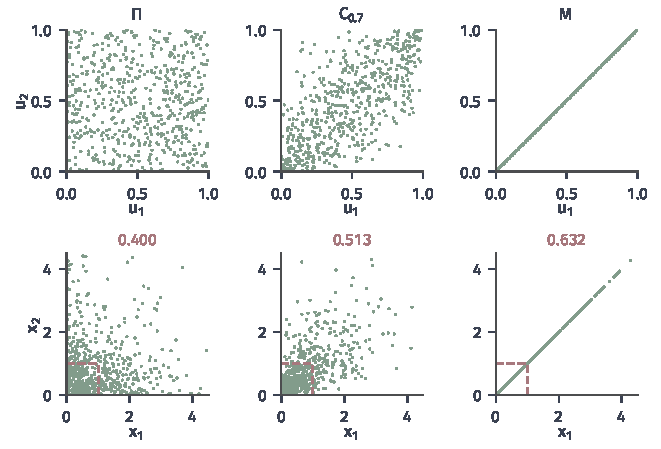
\includegraphics[width=112mm]{figures/07-probability/04-distribution-analysis/matplotlib/dfam-copula-samples/figure.pdf}
  \caption{同样的边缘，不同的依赖。上排：乘积Copula $\Pi$、$\rho=0.7$的高斯Copula、完全同向的$M$，各$600$个样本（绿，种子$716$）。下排：把上排每个点的两个坐标都用$u\mapsto-\ln(1-u)$变换，两个边缘都是$\operatorname{Exp}(1)$；红色虚线围出事件$\{X_1\leq1,X_2\leq1\}$，其概率依次约为$0.400$、$0.513$、$0.632$。}
  \label{fig:dfam-copula-samples}
\end{BookInlineFigure}

\paragraph{依赖的两个极端}
$M$与$W$分别是“完全同向”与“完全反向”的依赖，任何二元Copula都夹在它们之间。

\begin{lemma}[Fréchet–Hoeffding界]
\label{lem:dfam-frechet-bounds}
对任一二元Copula $C$与$u,v\in[0,1]$，
\begin{equation}
  W(u,v)\leq C(u,v)\leq M(u,v).
  \label{eq:dfam-frechet-bounds}
\end{equation}
\end{lemma}

\begin{proof}
设$(U_1,U_2)$的联合分布函数为$C$。事件$\{U_1\leq u,U_2\leq v\}$包含于$\{U_1\leq u\}$，也包含于$\{U_2\leq v\}$，所以$C(u,v)\leq u$且$C(u,v)\leq v$，即$C\leq M$。另一方面，由并集的概率公式，
\[
  C(u,v)=\mathbb{P}(U_1\leq u)+\mathbb{P}(U_2\leq v)-\mathbb{P}(U_1\leq u\text{或}U_2\leq v)\geq u+v-1 ,
\]
又$C(u,v)\geq0$，所以$C\geq W$。
\end{proof}

图~\ref{fig:dfam-copula-bounds}沿对角线比较几个Copula：$C(u,u)$是两个分量都不超过各自$u$分位数的概率。完全同向时它等于$u$，独立时是$u^{2}$，完全反向时在$u\leq1/2$以前一直为零。图中$u=0.632$处的四个值就是上面两台设备的四个概率。

\begin{BookInlineFigure}
  \centering
  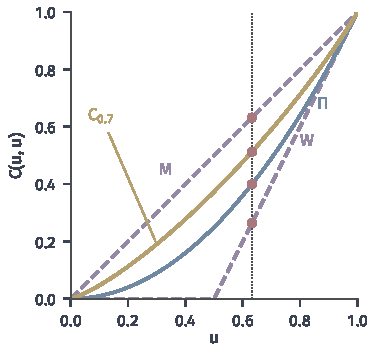
\includegraphics[width=64mm]{figures/07-probability/04-distribution-analysis/matplotlib/dfam-copula-bounds/figure.pdf}
  \caption{Copula在对角线上的取值$C(u,u)$。紫色虚线为上下界$M(u,u)=u$与$W(u,u)=\max(2u-1,0)$，蓝线为乘积Copula $u^{2}$，黄线为$\rho=0.7$的高斯Copula。红点标出$u=1-\mathrm{e}^{-1}\approx0.632$处的四个值$0.264,0.400,0.513,0.632$。}
  \label{fig:dfam-copula-bounds}
\end{BookInlineFigure}

\subsection{唯一性的范围}
\label{sec:dfam-copula-uniqueness}

现在反过来：给定$\bm{X}$的联合分布，能否找到它的Copula，找到的是否唯一？自然的想法是把每个分量用自己的分布函数送回$(0,1)$，令$U_i=F_i(X_i)$。这个想法在边缘连续时完全成立，在边缘有原子时会出问题。

\paragraph{连续边缘：概率积分变换}
先看一个分量。把$X$代入它自己的分布函数，得到$F(X)$，这个操作称为\term{概率积分变换}（probability integral transform）。

\begin{lemma}[概率积分变换]
\label{lem:dfam-pit}
设实值随机变量$X$的分布函数$F$连续。则$F(X)\sim\operatorname{Unif}(0,1)$，并且对每个$x$，事件$\{F(X)\leq F(x)\}$与$\{X\leq x\}$只差一个零概率事件。
\end{lemma}

\begin{proof}
记$Q$为$F$的分位数函数。对$u\in(0,1)$，由第~\ref{chap:random-variables}章的引理，$F(y)\geq u$当且仅当$y\geq Q(u)$，所以
\[
  \mathbb{P}\bigl(F(X)\geq u\bigr)=\mathbb{P}\bigl(X\geq Q(u)\bigr)=1-F\bigl(Q(u)-\bigr).
\]
另一方面，由同一引理有$F(Q(u))\geq u$；对$y<Q(u)$又有$F(y)<u$，令$y\uparrow Q(u)$得$F(Q(u)-)\leq u$。$F$连续，左极限等于函数值，两者合起来给出$F(Q(u))=u$。代入上式，
\[
  \mathbb{P}\bigl(F(X)\geq u\bigr)=1-u ,
\]
所以$F(X)$在$(0,1)$上均匀，又以概率$1$取值于$[0,1]$。

对第二个结论，$\{X\leq x\}\subseteq\{F(X)\leq F(x)\}$由单调性得到。差集是$\{X>x,\ F(X)=F(x)\}$，在其上$X$落在$F$取常值$F(x)$的区间里。记$b=\sup\{y:F(y)=F(x)\}$，这个事件包含于$\{x<X\leq b\}$（$b=+\infty$时为$\{X>x\}$），其概率是$F(b)-F(x)=0$（$b$有限时$F$连续，$F(b)=F(x)$；$b=+\infty$时$F(x)=1$）。
\end{proof}

\begin{proof}[Sklar定理第二部分的证明（边缘连续）]
设各$F_i$连续，令$U_i=F_i(X_i)$，$C$为$\bm{U}$的联合分布函数。由引理~\ref{lem:dfam-pit}，每个$U_i$均匀，$C$是Copula；且$\{U_i\leq F_i(x_i)\}$与$\{X_i\leq x_i\}$只差零概率事件，所以
\[
  C\bigl(F_1(x_1),\dots,F_d(x_d)\bigr)=\mathbb{P}(X_1\leq x_1,\dots,X_d\leq x_d)=F(x_1,\dots,x_d).
\]
唯一性：若$C'$也满足式~\eqref{eq:dfam-sklar}，则对每组$x_i$有$C'(F_1(x_1),\dots)=F(x_1,\dots)=C(F_1(x_1),\dots)$，所以$C'$与$C$在$\operatorname{Ran}F_1\times\cdots\times\operatorname{Ran}F_d$上相等。$F_i$连续时值域包含$(0,1)$，再由下面的引理~\ref{lem:dfam-copula-lipschitz}，$C$与$C'$都连续，于是在$[0,1]^{d}$上处处相等。
\end{proof}

\begin{lemma}[Copula的Lipschitz性]
\label{lem:dfam-copula-lipschitz}
对任一$d$元Copula $C$与$\bm{u},\bm{v}\in[0,1]^{d}$，
\begin{equation}
  \lvert C(\bm{u})-C(\bm{v})\rvert\leq\sum_{i=1}^{d}\lvert u_i-v_i\rvert .
  \label{eq:dfam-copula-lipschitz}
\end{equation}
\end{lemma}

\begin{proof}
设$\bm{U}$的联合分布函数为$C$。事件$\{\bm{U}\leq\bm{u}\}$与$\{\bm{U}\leq\bm{v}\}$的对称差中，至少有一个$i$使$U_i$落在$u_i$与$v_i$之间。由并集的概率不超过概率之和，
\[
  \lvert C(\bm{u})-C(\bm{v})\rvert\leq\sum_{i=1}^{d}\mathbb{P}\bigl(\min(u_i,v_i)<U_i\leq\max(u_i,v_i)\bigr)=\sum_{i=1}^{d}\lvert u_i-v_i\rvert ,
\]
最后一步用到$U_i$均匀。
\end{proof}

边缘连续时，唯一的Copula还有一个有用的性质。证明表明，这个Copula就是$(F_1(X_1),\dots,F_d(X_d))$的联合分布函数。设$g_1,\dots,g_d$都严格递增，$Y_i=g_i(X_i)$，其分布函数记为$G_i$。由$\{Y_i\leq g_i(x)\}=\{X_i\leq x\}$，
\[
  G_i\bigl(g_i(x)\bigr)=F_i(x),
\]
$G_i$也连续（$\mathbb{P}(Y_i=y)$不超过$X_i$取某个单点的概率，为零）。于是$G_i(Y_i)=F_i(X_i)$，$(Y_1,\dots,Y_d)$送回均匀刻度后得到的是同一个随机向量，Copula相同。分量各自作严格递增的重新刻度，Copula不变；依赖结构因此与单位、对数刻度这类选择无关，这正是“边缘以外的部分”应有的样子。

\paragraph{有原子时只在值域上唯一}
边缘有原子时，概率积分变换失效。取$X\sim\operatorname{Bern}(\tfrac12)$，$F(0)=\tfrac12$，$F(1)=1$，于是$F(X)$只取$\tfrac12$和$1$两个值，各有概率$\tfrac12$，根本不是均匀分布。图~\ref{fig:dfam-pit}(b)画出了这一点：质量在原子处不能被摊开；作为对照，(a)中连续的$\operatorname{Exp}(1)$经概率积分变换后确实均匀。

\begin{BookInlineFigure}
  \centering
  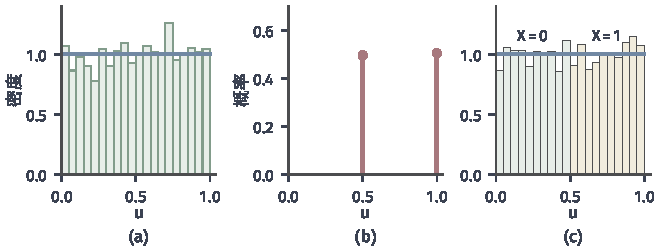
\includegraphics[width=112mm]{figures/07-probability/04-distribution-analysis/matplotlib/dfam-pit/figure.pdf}
  \caption{把分量送回均匀刻度，各$4000$个模拟值（种子$716$）。(a)$X\sim\operatorname{Exp}(1)$时$F(X)$的直方图（浅绿），蓝线是均匀密度$1$。(b)$X\sim\operatorname{Bern}(\frac12)$时$F(X)$只取$\frac12$与$1$（红色竖线，高度为概率）。(c)同一枚硬币的分布变换$U=F(X-)+V\Delta F(X)$：$X=0$的值摊在$(0,\frac12]$（浅绿），$X=1$的值摊在$(\frac12,1]$（浅黄），合起来是均匀分布。}
  \label{fig:dfam-pit}
\end{BookInlineFigure}

再看唯一性。设$X_1,X_2$是两枚独立的公平硬币。$\operatorname{Ran}F_i=\{0,\tfrac12,1\}$，式~\eqref{eq:dfam-sklar}只在这九个格点上约束$C$。$u$或$v$为$0$时任何Copula都取$0$，$u=1$时取$v$，$v=1$时取$u$，这些格点自动满足；真正的约束只有一个：
\[
  C(\tfrac12,\tfrac12)=\mathbb{P}(X_1=0,X_2=0)=\tfrac14 .
\]
乘积Copula满足它。$C'=\tfrac12M+\tfrac12W$也满足：两个Copula的凸组合仍是Copula（按权重混合两个均匀边缘的随机向量，边缘仍均匀），且
\[
  C'(\tfrac12,\tfrac12)=\tfrac12\cdot\tfrac12+\tfrac12\cdot0=\tfrac14 .
\]
可是在$(\tfrac14,\tfrac14)$处，$\Pi$取$\tfrac1{16}$，$C'$取$\tfrac12\cdot\tfrac14+0=\tfrac18$，两者不同。所以两枚独立硬币的联合分布既可以写成$\Pi(F_1,F_2)$，也可以写成$C'(F_1,F_2)$。

\begin{BookInlineFigure}
  \centering
  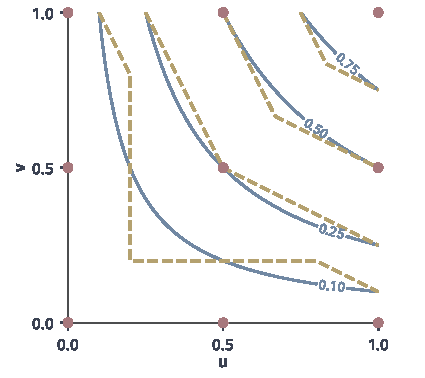
\includegraphics[width=72mm]{figures/07-probability/04-distribution-analysis/matplotlib/dfam-copula-atoms/figure.pdf}
  \caption{有原子时Copula只在值域格点上确定。两枚独立公平硬币，$\operatorname{Ran}F_1\times\operatorname{Ran}F_2$是九个格点（红点）。蓝色实线是乘积Copula $\Pi$的等值线，黄色虚线是$\frac12M+\frac12W$的等值线，层级为$0.1,0.25,0.5,0.75$；两族曲线在红点处取相同的值，在格点之间不同。}
  \label{fig:dfam-copula-atoms}
\end{BookInlineFigure}

图~\ref{fig:dfam-copula-atoms}画出这两个Copula的等值线：它们在九个红点上一致，在其他地方不同。这个例子说明，含原子时“从联合分布读出的Copula”并不唯一，不同的选择可能给人截然不同的依赖印象：$C'$看上去一半完全同向、一半完全反向，实际描述的却是两枚独立的硬币。连续情形的变换论证不能照搬，依据Copula谈论依赖时，必须先确认边缘是否连续。

\paragraph{有原子时的存在性}
唯一性失去了，存在性仍然成立。办法是在每个原子上用一个独立的均匀变量把质量摊开，这称为\term{分布变换}（distributional transform）。

\begin{lemma}[分布变换]
\label{lem:dfam-distributional-transform}
设$X$的分布函数为$F$，$V\sim\operatorname{Unif}(0,1)$与$X$独立，记$F(x-)$为左极限、$\Delta F(x)=F(x)-F(x-)$。令
\begin{equation}
  U=F(X-)+V\,\Delta F(X).
  \label{eq:dfam-distributional-transform}
\end{equation}
则$U\sim\operatorname{Unif}(0,1)$，并且对每个$x$，事件$\{U\leq F(x)\}$与$\{X\leq x\}$只差一个零概率事件。
\end{lemma}

\begin{proof}
固定$u\in(0,1)$，令$x_0=Q(u)$，则$F(x_0-)\leq u\leq F(x_0)$。由$V$与$X$独立，给定$X=y$时$U$在区间$[F(y-),F(y)]$上均匀（$\Delta F(y)=0$时退化为一点），所以
\[
  \mathbb{P}(U\leq u)=\mathbb{E}[g(X)],\qquad g(y)=\mathbb{P}\bigl(F(y-)+V\Delta F(y)\leq u\bigr).
\]
按$y$与$x_0$的位置分三种情形：
\begin{itemize}
  \item $y<x_0$：$F(y)\leq F(x_0-)\leq u$，$g(y)=1$，这部分贡献$\mathbb{P}(X<x_0)=F(x_0-)$。
  \item $y=x_0$：若$\Delta F(x_0)>0$，$g(x_0)=(u-F(x_0-))/\Delta F(x_0)$，贡献$\Delta F(x_0)\,g(x_0)=u-F(x_0-)$；若$\Delta F(x_0)=0$，则$F(x_0-)=u$，贡献为$0=u-F(x_0-)$。
  \item $y>x_0$：$F(y-)\geq F(x_0)\geq u$。$g(y)>0$只可能在$F(y-)=u$且$\Delta F(y)=0$时发生，这时$F(y)=F(x_0)$，$y$落在$F$取常值的区间里，这样的$y$整体的概率为零（与引理~\ref{lem:dfam-pit}的论证相同），贡献为$0$。
\end{itemize}
三部分相加，
\[
  \mathbb{P}(U\leq u)=F(x_0-)+\bigl(u-F(x_0-)\bigr)=u ,
\]
所以$U$均匀。

对第二个结论，$X\leq x$时$U\leq F(X)\leq F(x)$。$X>x$时$U\geq F(X-)\geq F(x)$，要使$U\leq F(x)$只能$U=F(x)=F(X-)$且$V\Delta F(X)=0$，即$V=0$，或者$\Delta F(X)=0$而$F(X)=F(x)$；前者概率为零，后者又是$X$落在$F$取常值的区间里，概率也为零。
\end{proof}

\begin{proof}[Sklar定理第二部分的证明（一般情形）]
取与$\bm{X}$独立的$V_1,\dots,V_d$，它们独立同分布于$\operatorname{Unif}(0,1)$，对每个分量按式~\eqref{eq:dfam-distributional-transform}作分布变换，得到$\bm{U}$，令$C$为它的联合分布函数。由引理~\ref{lem:dfam-distributional-transform}，$C$是Copula，且$\{U_i\leq F_i(x_i)\}$与$\{X_i\leq x_i\}$只差零概率事件，与连续情形一样得到式~\eqref{eq:dfam-sklar}。在$\operatorname{Ran}F_1\times\cdots\times\operatorname{Ran}F_d$上的唯一性，与连续情形的论证相同。
\end{proof}

分布变换在连续点上退化为$F(X)$，所以它是概率积分变换的推广。它得到的Copula依赖于为摊开原子而引入的独立变量$V_i$：图~\ref{fig:dfam-pit}(c)中，硬币的两个原子各被摊成长为$\tfrac12$的一段，两枚独立硬币配独立的$V_1,V_2$，得到的正是乘积Copula；若让$V_1=V_2$，就得到另一个同样合法的Copula。这再次说明含原子时Copula是联合分布的一种表示，而不是由它唯一决定的量。


\section{指数族}
\label{sec:dfam-exponential}

把Bernoulli、Poisson和高斯的概率公式取对数，会看到同一个结构。Bernoulli分布的对数质量是$x\ln\frac{p}{1-p}+\ln(1-p)$，Poisson分布是$x\ln\lambda-\lambda-\ln x!$，高斯分布是$x$与$x^{2}$的线性组合再加常数。三者都是“若干个统计量的线性组合，加上只依赖参数的归一化项，再加上只依赖$x$的项”。改变参数，就是改变给每个统计量的指数权重。

这一节先把这种形式写准，区分哪些对象固定、哪些随参数变化；再确定参数能取哪些值；然后看归一化项的导数怎样给出矩；最后把指数权重与它产生的均值对应起来。

\subsection{指数形式}
\label{sec:dfam-exponential-form}

\begin{definition}[指数族]
\label{def:dfam-exponential-family}
设$\nu$是$\mathcal{X}$上的$\sigma$有限测度，$h:\mathcal{X}\to[0,\infty)$与$\bm{T}:\mathcal{X}\to\mathbb{R}^{k}$可测，$\nu(\{h>0\})>0$。对使
\begin{equation}
  Z(\bm{\theta})=\int_{\mathcal{X}}h(x)\,\mathrm{e}^{\langle\bm{\theta},\bm{T}(x)\rangle}\,\nu(\mathrm{d}x)<\infty
  \label{eq:dfam-partition}
\end{equation}
的$\bm{\theta}\in\mathbb{R}^{k}$，令$A(\bm{\theta})=\ln Z(\bm{\theta})$，并以
\begin{equation}
  p_{\bm{\theta}}(x)=h(x)\exp\bigl(\langle\bm{\theta},\bm{T}(x)\rangle-A(\bm{\theta})\bigr)
  \label{eq:dfam-exponential-family}
\end{equation}
为相对$\nu$的密度定义$P_{\bm{\theta}}$。这样得到的分布族称为\term{指数族}（exponential family）。$\bm{T}$称为\term{自然统计量}（natural statistic），$\bm{\theta}$称为\term{自然参数}（natural parameter），$Z$与$A$分别称为\term{配分函数}（partition function）与\term{对数配分函数}（log-partition function）。
\end{definition}

式~\eqref{eq:dfam-exponential-family}中有三样东西是事先固定的：参考测度$\nu$、函数$h$和统计量$\bm{T}$。$h$与$\nu$只以乘积$h(x)\nu(\mathrm{d}x)$的形式出现，这个乘积称为\term{基准测度}（base measure），它决定哪些$x$可能出现，以及在不加任何指数权重时质量怎样分布。随参数变化的只有$\bm{\theta}$；$A(\bm{\theta})$不是另一个可以自由选择的量，它由归一化唯一确定，保证$p_{\bm{\theta}}$积分为$1$。

由式~\eqref{eq:dfam-exponential-family}，$p_{\bm{\theta}}(x)>0$当且仅当$h(x)>0$。所以指数族的所有成员有共同的支撑$\{h>0\}$，参数只改变支撑上质量的相对多少，不能把质量挪到$h$为零的地方。$\operatorname{Unif}(0,\theta)$的支撑随$\theta$变化，它就不能写成任何指数族。

\paragraph{三个分布的指数形式}
Bernoulli分布取$\nu$为$\{0,1\}$上的计数测度，
\[
  p^{x}(1-p)^{1-x}=\exp\Bigl(x\ln\frac{p}{1-p}+\ln(1-p)\Bigr).
\]
对照式~\eqref{eq:dfam-exponential-family}，$h=1$，$T(x)=x$，自然参数$\theta=\ln\frac{p}{1-p}$，即$p=\mathrm{e}^{\theta}/(1+\mathrm{e}^{\theta})$，再由$-A(\theta)=\ln(1-p)$得
\[
  A(\theta)=\ln(1+\mathrm{e}^{\theta}).
\]

Poisson分布取$\nu$为$\{0,1,2,\dots\}$上的计数测度，
\[
  \mathrm{e}^{-\lambda}\frac{\lambda^{x}}{x!}=\frac{1}{x!}\exp(x\ln\lambda-\lambda),
\]
所以$h(x)=1/x!$，$T(x)=x$，$\theta=\ln\lambda$，$A(\theta)=\mathrm{e}^{\theta}$。

高斯分布$\mathcal{N}(m,s^{2})$取$\nu$为Lebesgue测度，把指数中的平方展开：
\[
  \frac{1}{\sqrt{2\pi s^{2}}}\mathrm{e}^{-\frac{(x-m)^{2}}{2s^{2}}}=\frac{1}{\sqrt{2\pi}}\exp\Bigl(\frac{m}{s^{2}}x-\frac{1}{2s^{2}}x^{2}-\frac{m^{2}}{2s^{2}}-\ln s\Bigr).
\]
于是$h=1/\sqrt{2\pi}$，$\bm{T}(x)=(x,x^{2})$，自然参数是
\begin{equation}
  \bm{\theta}=(\theta_1,\theta_2)=\Bigl(\frac{m}{s^{2}},\ -\frac{1}{2s^{2}}\Bigr).
  \label{eq:dfam-gaussian-natural}
\end{equation}
反解得$s^{2}=-1/(2\theta_2)$，$m=-\theta_1/(2\theta_2)$，代入$\frac{m^{2}}{2s^{2}}+\ln s$，得到
\begin{equation}
  A(\bm{\theta})=-\frac{\theta_1^{2}}{4\theta_2}-\frac12\ln(-2\theta_2).
  \label{eq:dfam-gaussian-log-partition}
\end{equation}

\paragraph{同一个分布的不同写法}
指数形式不是唯一的。把高斯的统计量换成$\bm{T}'(x)=(x,-x^{2}/2)$，自然参数就变成$(m/s^{2},\ 1/s^{2})$；常数$1/\sqrt{2\pi}$也可以从$h$移进$A$。一般地，统计量作可逆线性变换$\bm{T}'=\bm{L}\bm{T}$，自然参数就作相应的变换$\bm{\theta}'=\bm{L}^{-\top}\bm{\theta}$，于是
\[
  \langle\bm{\theta}',\bm{T}'\rangle=\bm{\theta}^{\top}\bm{L}^{-1}\bm{L}\bm{T}=\langle\bm{\theta},\bm{T}\rangle ,
\]
指数不变，分布族也不变。

所以“自然参数”是相对于选定的$\bm{T}$与$h\nu$而言的，不能把密度公式里出现的任意参数都叫作自然参数。高斯族的均值$m$在式~\eqref{eq:dfam-gaussian-natural}中与$s^{2}$纠缠在一起，又出现在$A$里，它不是这组表示下的自然参数。但若只看方差固定为$1$的子族$\{\mathcal{N}(m,1)\}$，取$h=\varphi$、$T(x)=x$，则
\[
  \varphi(x-m)=\varphi(x)\exp\bigl(mx-\tfrac12m^{2}\bigr),
\]
$m$恰好是自然参数，$A(m)=m^{2}/2$。同一个数字是否是自然参数，取决于整个表示。

写法还可能带来冗余。Bernoulli分布也可以写成
\[
  p^{x}(1-p)^{1-x}=\exp\bigl(\theta_0\mathbf{1}_{\{x=0\}}+\theta_1\mathbf{1}_{\{x=1\}}\bigr),\qquad(\theta_0,\theta_1)=(\ln(1-p),\ln p).
\]
两个统计量之和恒为$1$，把$(\theta_0,\theta_1)$同时加上同一个常数，归一化后分布不变。这种冗余与第~\ref{sec:dfam-identifiability}节的重复参数是同一回事，后面两小节会精确地描述它。

\subsection{自然参数域}
\label{sec:dfam-natural-domain}

式~\eqref{eq:dfam-exponential-family}只在$Z(\bm{\theta})$有限且为正时才定义了概率分布。被积函数在$\{h>0\}$上为正，而$\nu(\{h>0\})>0$，所以$Z(\bm{\theta})>0$总成立；问题只在于是否有限。

\begin{definition}[自然参数域]
\label{def:dfam-natural-domain}
集合
\begin{equation}
  \Theta=\{\bm{\theta}\in\mathbb{R}^{k}:Z(\bm{\theta})<\infty\}
  \label{eq:dfam-natural-domain}
\end{equation}
称为指数族的\term{自然参数域}（natural parameter space）。若$\Theta$是$\mathbb{R}^{k}$中的开集，称这个指数族是\term{正则指数族}（regular exponential family）。
\end{definition}

$\Theta$以外的$\bm{\theta}$给出的表达式$h\,\mathrm{e}^{\langle\bm{\theta},\bm{T}\rangle}$不能归一化，它只是一个形式表达式，不是概率分布。例如在$(0,\infty)$上取$h=1$、$T(x)=x$，$\int_0^\infty\mathrm{e}^{\theta x}\,\mathrm{d}x$在$\theta<0$时等于$-1/\theta$，在$\theta\geq0$时发散。所以$\Theta=(-\infty,0)$，$\theta=-\lambda$对应$\operatorname{Exp}(\lambda)$，$A(\theta)=-\ln(-\theta)$。

\begin{lemma}[自然参数域的凸性]
\label{lem:dfam-domain-convex}
$\Theta$是凸集，$A$是$\Theta$上的凸函数。
\end{lemma}

\begin{proof}
设$\bm{\theta},\bm{\theta}'\in\Theta$，$0<\lambda<1$。被积函数可以拆成两个幂的乘积：
\[
  \mathrm{e}^{\langle\lambda\bm{\theta}+(1-\lambda)\bm{\theta}',\bm{T}\rangle}=\bigl(\mathrm{e}^{\langle\bm{\theta},\bm{T}\rangle}\bigr)^{\lambda}\bigl(\mathrm{e}^{\langle\bm{\theta}',\bm{T}\rangle}\bigr)^{1-\lambda}.
\]
对测度$h\nu$用指数为$1/\lambda$与$1/(1-\lambda)$的Hölder不等式（见\BookChapterRef{chap:function-normed-spaces}{卷四第11章“赋范空间”}），
\[
  Z\bigl(\lambda\bm{\theta}+(1-\lambda)\bm{\theta}'\bigr)\leq Z(\bm{\theta})^{\lambda}Z(\bm{\theta}')^{1-\lambda}<\infty .
\]
所以$\lambda\bm{\theta}+(1-\lambda)\bm{\theta}'\in\Theta$。两边取对数，得到
\[
  A\bigl(\lambda\bm{\theta}+(1-\lambda)\bm{\theta}'\bigr)\leq\lambda A(\bm{\theta})+(1-\lambda)A(\bm{\theta}') .
\]
\end{proof}

\paragraph{几个参数域}
Bernoulli与Poisson的配分和对任何$\theta$都有限，$\Theta=\mathbb{R}$。高斯族的配分积分是
\[
  Z(\bm{\theta})=\frac{1}{\sqrt{2\pi}}\int_{-\infty}^{\infty}\mathrm{e}^{\theta_1x+\theta_2x^{2}}\,\mathrm{d}x ,
\]
它在$\theta_2<0$时有限；$\theta_2=0$时被积函数是$\mathrm{e}^{\theta_1x}$，在某一侧不衰减；$\theta_2>0$时在两侧都发散。所以$\Theta=\{(\theta_1,\theta_2):\theta_2<0\}$是开半平面，高斯族是正则的。

自然参数域不一定是开的。在$(0,\infty)$上取$h(x)=(1+x)^{-2}$、$T(x)=x$，
\[
  Z(\theta)=\int_0^\infty\frac{\mathrm{e}^{\theta x}}{(1+x)^{2}}\,\mathrm{d}x .
\]
$\theta>0$时被积函数趋于无穷，积分发散；$\theta\leq0$时被积函数不超过$(1+x)^{-2}$，积分有限，且$Z(0)=1$。所以$\Theta=(-\infty,0]$，边界点$0$属于参数域，它对应的分布就是密度$(1+x)^{-2}$。这个分布的均值是$\int_0^\infty x(1+x)^{-2}\,\mathrm{d}x=\infty$。

图~\ref{fig:dfam-natural-domain}比较这两个一维的例子。指数分布族的$A(\theta)$在$\theta\uparrow0$时趋于无穷，参数域在$0$处断开；第二个族的$A(\theta)$在$0$处取有限值$0$，但均值$\mathbb{E}_\theta[X]$在$\theta\uparrow0$时趋于无穷，曲线在边界处变得竖直。边界点属于参数域，并不意味着那里的分布与内部一样好用：它的均值已经不存在了，下一小节的导数公式在那里不成立。

\begin{BookInlineFigure}
  \centering
  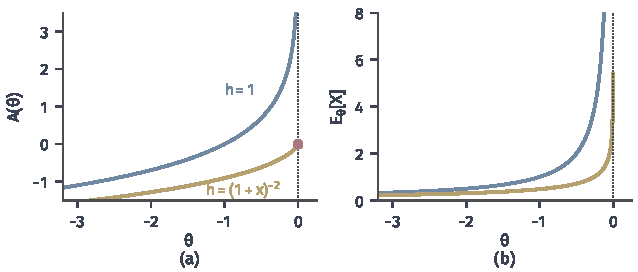
\includegraphics[width=108mm]{figures/07-probability/04-distribution-analysis/matplotlib/dfam-natural-domain/figure.pdf}
  \caption{两个一维指数族的自然参数域，$T(x)=x$，$x>0$。蓝：$h=1$（指数分布族），$\Theta=(-\infty,0)$；黄：$h(x)=(1+x)^{-2}$，$\Theta=(-\infty,0]$，红点是属于参数域的边界点$\theta=0$。(a)对数配分函数$A(\theta)$。(b)均值$\mathbb{E}_\theta[X]$，两者在$\theta\uparrow0$时都趋于无穷。黄线由数值积分得到。}
  \label{fig:dfam-natural-domain}
\end{BookInlineFigure}

\paragraph{退化的极限}
参数趋于无穷时，分布可能趋于族外的分布。在$\{0,1,2\}$上取计数测度、$h=1$、$T(x)=x$，得到一个单参数指数族
\begin{equation}
  p_\theta(x)=\frac{\mathrm{e}^{\theta x}}{1+\mathrm{e}^{\theta}+\mathrm{e}^{2\theta}},\qquad x=0,1,2,\quad\theta\in\mathbb{R}.
  \label{eq:dfam-tilt}
\end{equation}
它从均匀表出发，按$\mathrm{e}^{\theta x}$给较大的点数加权：$\theta=0$时是均匀表，$\theta=\ln2$时权重为$1,2,4$，
\[
  p_{\ln2}=\bigl(\tfrac17,\ \tfrac27,\ \tfrac47\bigr).
\]
$\theta\to+\infty$时，分子分母同除以$\mathrm{e}^{2\theta}$，$p_\theta(2)\to1$，分布趋于点质量$\delta_2$；$\theta\to-\infty$时趋于$\delta_0$。

但$\delta_2$不等于任何$p_\theta$，因为每个$p_\theta$在三个点上都为正。图~\ref{fig:dfam-tilt-simplex}把这个族画在第~\ref{sec:dfam-candidates}节的三角形中：它是穿过内部的一条曲线，两端无限接近顶点而不到达。族的闭包含有边界上的分布，而这些分布不能用有限的自然参数表示。

\begin{BookInlineFigure}
  \centering
  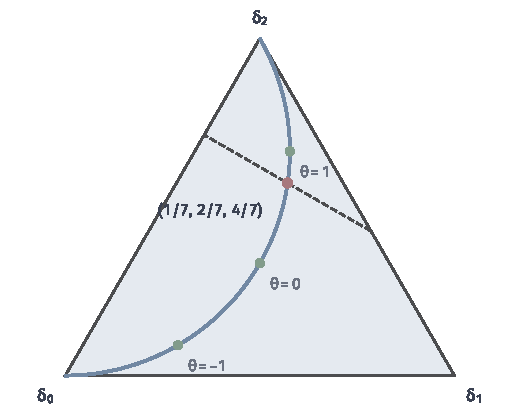
\includegraphics[width=88mm]{figures/07-probability/04-distribution-analysis/matplotlib/dfam-tilt-simplex/figure.pdf}
  \caption{式~\eqref{eq:dfam-tilt}的单参数指数族在三角形$\Delta_2$中的轨迹（蓝线），$\theta$从$-6$到$6$。绿点依次是$\theta=-1,0,1$，红点是$\theta=\ln2$对应的$(\frac17,\frac27,\frac47)$；曲线两端趋于顶点$\delta_0$与$\delta_2$，但不到达。深灰虚线是满足$\mathbb{E}_P[X]=\frac{10}{7}$的全部概率表，它与曲线只交于红点。}
  \label{fig:dfam-tilt-simplex}
\end{BookInlineFigure}

\subsection{配分函数的导数}
\label{sec:dfam-partition-derivatives}

对数配分函数原本只是为归一化而设，但它把整个族的矩都存了起来。对式~\eqref{eq:dfam-partition}关于$\theta_j$求导，形式上会在积分号内落下一个因子$T_j(x)$，这正是$T_j$的期望。下面的定理说明，在参数域内部这个形式计算是合法的。

\begin{theorem}[对数配分函数的导数]
\label{thm:dfam-log-partition-derivatives}
设$\bm{\theta}$是$\Theta$的内点。则在$P_{\bm{\theta}}$下$\bm{T}$的各分量有任意阶矩，$A$在$\bm{\theta}$处二阶可微，且
\begin{equation}
  \nabla A(\bm{\theta})=\mathbb{E}_{\bm{\theta}}[\bm{T}],\qquad\nabla^{2}A(\bm{\theta})=\operatorname{Cov}_{\bm{\theta}}(\bm{T}).
  \label{eq:dfam-log-partition-derivatives}
\end{equation}
\end{theorem}

\begin{proof}
取$\varepsilon>0$，使立方体$K=\bm{\theta}+[-2\varepsilon,2\varepsilon]^{k}$含于$\Theta$。函数$\bm{\eta}\mapsto\mathrm{e}^{\langle\bm{\eta},\bm{T}(x)\rangle}$是凸的，它在立方体$K$上的最大值在某个顶点处取到，所以对$\bm{\eta}\in K$，
\[
  \mathrm{e}^{\langle\bm{\eta},\bm{T}(x)\rangle}\leq G(x)=\sum_{\bm{v}}\mathrm{e}^{\langle\bm{v},\bm{T}(x)\rangle},
\]
其中$\bm{v}$取遍$K$的$2^{k}$个顶点。每个顶点都在$\Theta$中，所以$G$对$h\nu$可积。

再把统计量的多项式因子吸收进指数。由$\mathrm{e}^{s}\geq s$与$\mathrm{e}^{s}\geq s^{2}/2$（$s\geq0$），对实数$t$有
\[
  \lvert t\rvert\leq\frac{\mathrm{e}^{\varepsilon t}+\mathrm{e}^{-\varepsilon t}}{\varepsilon},\qquad t^{2}\leq\frac{2(\mathrm{e}^{\varepsilon t}+\mathrm{e}^{-\varepsilon t})}{\varepsilon^{2}} .
\]
设$\bm{\theta}'\in\bm{\theta}+[-\varepsilon,\varepsilon]^{k}$，则$\bm{\theta}'\pm\varepsilon\bm{e}_j\in K$。取$t=T_j(x)$，第二个不等式给出
\[
  T_j(x)^{2}\,\mathrm{e}^{\langle\bm{\theta}',\bm{T}(x)\rangle}\leq\frac{2}{\varepsilon^{2}}\bigl(\mathrm{e}^{\langle\bm{\theta}'+\varepsilon\bm{e}_j,\bm{T}\rangle}+\mathrm{e}^{\langle\bm{\theta}'-\varepsilon\bm{e}_j,\bm{T}\rangle}\bigr)\leq\frac{4}{\varepsilon^{2}}G(x).
\]
用第一个不等式同样得到
\[
  \lvert T_j\rvert\,\mathrm{e}^{\langle\bm{\theta}',\bm{T}\rangle}\leq\frac{2}{\varepsilon}G ,
\]
而由$\lvert T_iT_j\rvert\leq(T_i^{2}+T_j^{2})/2$，交叉项也被$4G/\varepsilon^{2}$控制。对更高的$r$次幂，由$\mathrm{e}^{s}\geq s^{r}/r!$（$s\geq0$）同样把$\lvert T_j\rvert^{r}$吸收进指数，得到任意阶矩有限。

有了与$\bm{\theta}'$无关的可积控制函数，由中值定理与控制收敛定理，可以在积分号下对$Z$求一阶和二阶偏导数（见\BookChapterRef{chap:integration}{卷四第6章“积分”}）：
\[
  \partial_jZ(\bm{\theta})=\int T_j\,h\,\mathrm{e}^{\langle\bm{\theta},\bm{T}\rangle}\,\mathrm{d}\nu,\qquad\partial_i\partial_jZ(\bm{\theta})=\int T_iT_j\,h\,\mathrm{e}^{\langle\bm{\theta},\bm{T}\rangle}\,\mathrm{d}\nu ,
\]
并且这些偏导数在$\bm{\theta}$附近连续。

除以$Z(\bm{\theta})$，就是$P_{\bm{\theta}}$下的期望：
\[
  \frac{\partial_jZ}{Z}=\mathbb{E}_{\bm{\theta}}[T_j],\qquad\frac{\partial_i\partial_jZ}{Z}=\mathbb{E}_{\bm{\theta}}[T_iT_j].
\]
由$A=\ln Z$，一阶偏导数是
\[
  \partial_jA=\frac{\partial_jZ}{Z}=\mathbb{E}_{\bm{\theta}}[T_j].
\]
再求一次导，
\[
  \partial_i\partial_jA=\frac{\partial_i\partial_jZ}{Z}-\frac{\partial_iZ\,\partial_jZ}{Z^{2}}=\mathbb{E}_{\bm{\theta}}[T_iT_j]-\mathbb{E}_{\bm{\theta}}[T_i]\,\mathbb{E}_{\bm{\theta}}[T_j].
\]
这就是$\operatorname{Cov}_{\bm{\theta}}(T_i,T_j)$。
\end{proof}

定理只对内点成立。上一小节的边界点$\theta=0$处，$\mathbb{E}_0[X]=\infty$，一阶导数公式已经失去意义。

\paragraph{例子中的导数}
Bernoulli族$A(\theta)=\ln(1+\mathrm{e}^{\theta})$，求导得
\[
  A'(\theta)=\frac{\mathrm{e}^{\theta}}{1+\mathrm{e}^{\theta}}=p,\qquad A''(\theta)=p(1-p),
\]
正是$\operatorname{Bern}(p)$的均值与方差。Poisson族$A(\theta)=\mathrm{e}^{\theta}=\lambda$，一阶、二阶导数都等于$\lambda$，均值与方差相等。

高斯族对式~\eqref{eq:dfam-gaussian-log-partition}求偏导，再用$m=-\theta_1/(2\theta_2)$与$s^{2}=-1/(2\theta_2)$换回去，
\[
  \frac{\partial A}{\partial\theta_1}=-\frac{\theta_1}{2\theta_2}=m,\qquad\frac{\partial A}{\partial\theta_2}=\frac{\theta_1^{2}}{4\theta_2^{2}}-\frac{1}{2\theta_2}=m^{2}+s^{2}.
\]
这正是$\mathbb{E}[X]$与$\mathbb{E}[X^{2}]$，与$\bm{T}=(x,x^{2})$对应。

对式~\eqref{eq:dfam-tilt}的族，对数配分函数是
\[
  A(\theta)=\ln\bigl(1+\mathrm{e}^{\theta}+\mathrm{e}^{2\theta}\bigr).
\]
在$\theta=\ln2$处，$\mathrm{e}^{\theta}=2$，
\[
  A(\ln2)=\ln7,\qquad A'(\ln2)=\frac{2+2\cdot4}{7}=\frac{10}{7}.
\]
再算二阶矩$\mathbb{E}[X^{2}]=(2+4\cdot4)/7=18/7$，于是
\[
  A''(\ln2)=\frac{18}{7}-\Bigl(\frac{10}{7}\Bigr)^{2}=\frac{26}{49}\approx0.531 .
\]
图~\ref{fig:dfam-log-partition}(a)中，红点处切线的斜率$10/7$就是这个分布的均值；(b)画出均值$A'(\theta)$与方差$A''(\theta)$随$\theta$的变化：均值从$0$单调升到$2$，方差在均值经过$1$时最大，在两端趋于零。

\begin{BookInlineFigure}
  \centering
  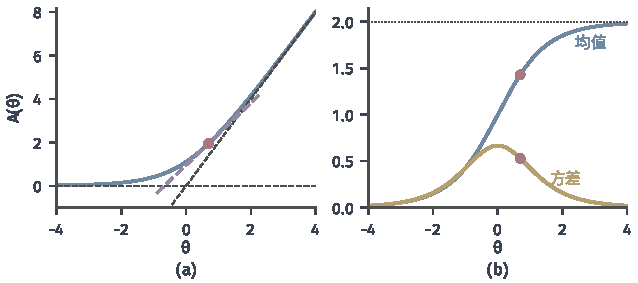
\includegraphics[width=108mm]{figures/07-probability/04-distribution-analysis/matplotlib/dfam-log-partition/figure.pdf}
  \caption{式~\eqref{eq:dfam-tilt}的对数配分函数。(a)$A(\theta)=\ln(1+\mathrm{e}^{\theta}+\mathrm{e}^{2\theta})$（蓝），红点$\theta=\ln2$处的切线（紫色虚线）斜率为$10/7$；两条深灰虚线是渐近线$y=0$与$y=2\theta$。(b)均值$A'(\theta)$（蓝）与方差$A''(\theta)$（黄），红点为$(\ln2,10/7)$与$(\ln2,26/49)$。}
  \label{fig:dfam-log-partition}
\end{BookInlineFigure}

\paragraph{累积量}
导数还能继续求下去。对$\bm{\theta}\in\Theta$与使$\bm{\theta}+\bm{t}\in\Theta$的$\bm{t}$，
\begin{equation}
  \ln\mathbb{E}_{\bm{\theta}}\bigl[\mathrm{e}^{\langle\bm{t},\bm{T}\rangle}\bigr]=\ln\frac{Z(\bm{\theta}+\bm{t})}{Z(\bm{\theta})}=A(\bm{\theta}+\bm{t})-A(\bm{\theta}).
  \label{eq:dfam-cumulant}
\end{equation}
左边是$\bm{T}$的矩母函数的对数，称为\term{累积量生成函数}（cumulant generating function）。式~\eqref{eq:dfam-cumulant}说明，在一个内点处，它就是把$A$平移到原点。$\bm{T}$在$P_{\bm{\theta}}$下的全部高阶矩信息，都由$A$在$\bm{\theta}$附近的形状给出。

\paragraph{凸性与仿射冗余}
由式~\eqref{eq:dfam-log-partition-derivatives}，对任意$\bm{a}\in\mathbb{R}^{k}$，
\[
  \bm{a}^{\top}\nabla^{2}A(\bm{\theta})\,\bm{a}=\operatorname{Var}_{\bm{\theta}}\bigl(\langle\bm{a},\bm{T}\rangle\bigr)\geq0 ,
\]
Hessian半正定，与引理~\ref{lem:dfam-domain-convex}的凸性相符。等号成立当且仅当$\langle\bm{a},\bm{T}\rangle$在$P_{\bm{\theta}}$下几乎必然为常数。

$P_{\bm{\theta}}$的密度在$\{h>0\}$上为正，所以$P_{\bm{\theta}}$与基准测度$h\nu$有相同的零测集，“$P_{\bm{\theta}}$下几乎必然”就是“$h\nu$下几乎处处”，与$\bm{\theta}$无关。于是Hessian在某个内点退化，当且仅当存在$\bm{a}\neq\bm{0}$与常数$c$，使
\begin{equation}
  \langle\bm{a},\bm{T}(x)\rangle=c\qquad\text{对}h\nu\text{几乎所有}x ,
  \label{eq:dfam-affine-redundancy}
\end{equation}
而这时它在所有内点处同时退化。式~\eqref{eq:dfam-affine-redundancy}说的是统计量之间有仿射关系，有一个分量是多余的。

第~\ref{sec:dfam-exponential-form}节Bernoulli的冗余写法正是如此：两个示性统计量满足$T_0+T_1=1$，取$\bm{a}=(1,1)$、$c=1$。这时
\[
  A(\bm{\theta})=\ln(\mathrm{e}^{\theta_0}+\mathrm{e}^{\theta_1}),\qquad A\bigl(\bm{\theta}+c'(1,1)\bigr)=A(\bm{\theta})+c',
\]
$A$沿$(1,1)$方向是线性的，不是严格凸的；而分布只依赖$\theta_1-\theta_0=\ln\frac{p}{1-p}$，沿这个方向完全不变。图~\ref{fig:dfam-overcomplete}画出这一点。

\begin{BookInlineFigure}
  \centering
  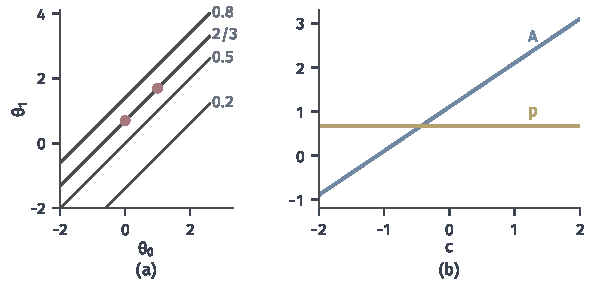
\includegraphics[width=100mm]{figures/07-probability/04-distribution-analysis/matplotlib/dfam-overcomplete/figure.pdf}
  \caption{Bernoulli族的冗余表示$\bm{T}=(\mathbf{1}_{\{x=0\}},\mathbf{1}_{\{x=1\}})$。(a)$(\theta_0,\theta_1)$平面中，分布相同的参数构成平行于$(1,1)$的直线（深灰），标注为对应的$p$；红点$(0,\ln2)$与$(1,1+\ln2)$都给出$p=\frac23$。(b)沿红点所在直线$\bm{\theta}=(0,\ln2)+c(1,1)$，$A$随$c$线性增长（蓝），而$p$保持$\frac23$（黄）。}
  \label{fig:dfam-overcomplete}
\end{BookInlineFigure}

\subsection{自然参数与均值参数}
\label{sec:dfam-natural-mean}

上一小节表明，Hessian退化与参数冗余是同一个现象。把统计量中多余的分量去掉，参数就不再冗余，而$\nabla A$给出的均值成为另一套可以替代自然参数的坐标。

\begin{definition}[最小表示与均值参数]
\label{def:dfam-minimal}
若不存在$\bm{a}\neq\bm{0}$与常数$c$使式~\eqref{eq:dfam-affine-redundancy}成立，则称指数族的这个表示是\term{最小表示}（minimal representation）。对$\bm{\theta}\in\Theta$，若$\mathbb{E}_{\bm{\theta}}[\bm{T}]$存在，称
\begin{equation}
  \bm{m}(\bm{\theta})=\mathbb{E}_{\bm{\theta}}[\bm{T}]
  \label{eq:dfam-mean-parameter}
\end{equation}
为$P_{\bm{\theta}}$的\term{均值参数}（mean parameter），$\bm{\theta}\mapsto\bm{m}(\bm{\theta})$称为\term{均值映射}（mean map）。
\end{definition}

在正则族中，每个$\bm{\theta}$都是内点，由定理~\ref{thm:dfam-log-partition-derivatives}，均值映射就是$\nabla A$。

\begin{theorem}[自然参数与均值参数的对应]
\label{thm:dfam-natural-mean}
设指数族采用最小表示。
\begin{enumerate}
  \item 参数化$\bm{\theta}\mapsto P_{\bm{\theta}}$在$\Theta$上可辨识。反之，若表示不是最小的，则参数化不可辨识。
  \item 若族还是正则的，则均值映射$\bm{m}=\nabla A$在$\Theta$上是单射，其Jacobian矩阵$\nabla^{2}A(\bm{\theta})$正定；像集$\mathcal{M}^{\circ}=\nabla A(\Theta)$是开集，逆映射$\mathcal{M}^{\circ}\to\Theta$连续可微。
  \item 在第二部分的条件下，若$\bm{a}\neq\bm{0}$且$\langle\bm{a},\bm{T}\rangle\leq c$对$h\nu$几乎所有$x$成立，则对每个$\bm{m}\in\mathcal{M}^{\circ}$有$\langle\bm{a},\bm{m}\rangle<c$。
\end{enumerate}
\end{theorem}

\begin{proof}
第一部分。设$P_{\bm{\theta}}=P_{\bm{\theta}'}$，则两个密度在$h\nu$下几乎处处相等。在$\{h>0\}$上取对数，得到
\[
  \langle\bm{\theta}-\bm{\theta}',\bm{T}(x)\rangle=A(\bm{\theta})-A(\bm{\theta}')\qquad\text{对}h\nu\text{几乎所有}x .
\]
这是形如式~\eqref{eq:dfam-affine-redundancy}的关系，$\bm{a}=\bm{\theta}-\bm{\theta}'$。最小表示排除了$\bm{a}\neq\bm{0}$，所以$\bm{\theta}=\bm{\theta}'$。

反之，若式~\eqref{eq:dfam-affine-redundancy}对某个$\bm{a}\neq\bm{0}$成立，取$\bm{\theta}\in\Theta$与$t\neq0$。在$h\nu$下几乎处处有
\[
  \mathrm{e}^{\langle\bm{\theta}+t\bm{a},\bm{T}\rangle}=\mathrm{e}^{tc}\,\mathrm{e}^{\langle\bm{\theta},\bm{T}\rangle},
\]
两边积分，
\[
  Z(\bm{\theta}+t\bm{a})=\mathrm{e}^{tc}Z(\bm{\theta})<\infty ,
\]
所以$\bm{\theta}+t\bm{a}\in\Theta$。两个密度中的因子$\mathrm{e}^{tc}$被归一化抵消，$P_{\bm{\theta}+t\bm{a}}=P_{\bm{\theta}}$，参数化不可辨识。

第二部分。由上一小节，最小表示下$\nabla^{2}A(\bm{\theta})$对每个$\bm{\theta}\in\Theta$正定。设$\bm{\theta}\neq\bm{\theta}'$，令$g(t)=A(\bm{\theta}'+t(\bm{\theta}-\bm{\theta}'))$，$t\in[0,1]$。$\Theta$凸，线段在$\Theta$内，
\[
  g''(t)=(\bm{\theta}-\bm{\theta}')^{\top}\nabla^{2}A\,(\bm{\theta}-\bm{\theta}')>0 ,
\]
所以$g'$严格递增，$g'(1)>g'(0)$，即
\[
  \bigl\langle\nabla A(\bm{\theta})-\nabla A(\bm{\theta}'),\ \bm{\theta}-\bm{\theta}'\bigr\rangle>0 .
\]
这说明$\nabla A(\bm{\theta})\neq\nabla A(\bm{\theta}')$，均值映射是单射。定理~\ref{thm:dfam-log-partition-derivatives}的证明给出$\nabla A$连续可微，Jacobian矩阵$\nabla^{2}A$正定因而可逆。由反函数定理（见\BookChapterRef{chap:implicit-inverse-functions}{卷二第22章“隐函数与反函数”}），$\nabla A$把每个点的一个邻域连续可微地一一映到一个开集上，于是像集$\mathcal{M}^{\circ}$是开集；结合全局单射，这些局部逆拼成一个连续可微的全局逆。

第三部分。设$\bm{m}=\nabla A(\bm{\theta})$且$\langle\bm{a},\bm{m}\rangle=c$。则$c-\langle\bm{a},\bm{T}\rangle$在$P_{\bm{\theta}}$下几乎必然非负，期望为零，所以几乎必然为零，也就是在$h\nu$下几乎处处有$\langle\bm{a},\bm{T}\rangle=c$，与最小表示矛盾。而$\langle\bm{a},\bm{m}\rangle\leq c$由期望的保序得到，所以严格不等式成立。
\end{proof}

第三部分说的是：统计量的取值被一个半空间$\{\langle\bm{a},\bm{t}\rangle\leq c\}$围住时，族中任何分布的均值都严格落在半空间内部，碰不到边界。边界上的均值只能由把全部质量放在超平面$\{\langle\bm{a},\bm{t}\rangle=c\}$上的分布实现，而指数族的成员都与基准测度有相同的零测集，做不到这一点。

\paragraph{三个例子}
Bernoulli族是最小表示，均值参数就是$p$。所有$\{0,1\}$上分布的均值组成$[0,1]$，均值映射的像却只是$(0,1)$：端点$0$与$1$是$\delta_0$与$\delta_1$的均值，它们不在族中，与第三部分（取$\bm{a}=\pm1$）一致。

式~\eqref{eq:dfam-tilt}的族中，均值映射$A'$把$\mathbb{R}$一一映到$(0,2)$。给定均值，可以反解自然参数。设均值为$10/7$，记$r=\mathrm{e}^{\theta}$，方程$A'(\theta)=10/7$是
\[
  \frac{r+2r^{2}}{1+r+r^{2}}=\frac{10}{7}.
\]
去分母并整理，得到
\[
  4r^{2}-3r-10=0 .
\]
它的正根是$r=(3+13)/8=2$（另一根$-5/4$为负，舍去），所以$\theta=\ln2$，回到$(\tfrac17,\tfrac27,\tfrac47)$。图~\ref{fig:dfam-tilt-simplex}中，这就是深灰虚线与曲线的交点。

高斯族中，均值参数是$(\mathbb{E}[X],\mathbb{E}[X^{2}])=(m,m^{2}+s^{2})$。由$s^{2}>0$，像集是抛物线上方的开区域
\[
  \mathcal{M}^{\circ}=\{(\eta_1,\eta_2):\eta_2>\eta_1^{2}\}.
\]
抛物线$\eta_2=\eta_1^{2}$本身对应方差为零的点质量，也是一切实值分布的$(\mathbb{E}[X],\mathbb{E}[X^{2}])$可以达到、指数族却达不到的边界。逆映射是$m=\eta_1$、$s^{2}=\eta_2-\eta_1^{2}$，代入式~\eqref{eq:dfam-gaussian-natural}即回到自然参数。例如$\bm{\theta}=(1,-\tfrac12)$对应$\mathcal{N}(1,1)$，均值参数是$(1,2)$。图~\ref{fig:dfam-mean-map}画出这对坐标之间的对应。

\begin{BookInlineFigure}
  \centering
  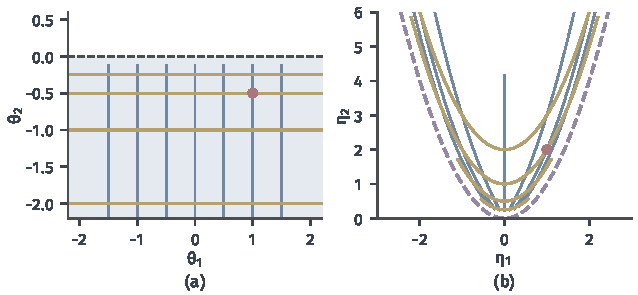
\includegraphics[width=108mm]{figures/07-probability/04-distribution-analysis/matplotlib/dfam-mean-map/figure.pdf}
  \caption{高斯族的自然参数与均值参数。(a)自然参数域是半平面$\theta_2<0$（浅蓝），画出直线族$\theta_1=$常数（蓝）与$\theta_2=$常数（黄）。(b)它们经$\nabla A$映到抛物线$\eta_2=\eta_1^{2}$（紫色虚线）上方的区域。红点是$\mathcal{N}(1,1)$：$\bm{\theta}=(1,-\frac12)$，$\bm{\eta}=(1,2)$。抛物线本身对应点质量，不在像中。}
  \label{fig:dfam-mean-map}
\end{BookInlineFigure}

\paragraph{对应的范围}
定理~\ref{thm:dfam-natural-mean}的坐标对应只在正则族的参数域与均值映射的像$\mathcal{M}^{\circ}$之间成立。它不覆盖可行均值的边界，也不覆盖非正则族的边界参数：第~\ref{sec:dfam-natural-domain}节中$h=(1+x)^{-2}$的族，边界点$\theta=0$在参数域中，那里却没有有限的均值参数。给定一个均值时是否存在族中的分布、存在时怎样求出对应的自然参数，以及在$\mathcal{M}^{\circ}$之外怎样处理，是第~\ref{chap:distribution-selection}章矩匹配的问题；两套坐标之间更细的几何关系由第~\ref{chap:information-geometry}章展开。


\section{本章小结}
\label{sec:dfam-summary}

章首的问题是：在挑选一个分布之前，怎样说清允许哪些分布、怎样给它们编号。第一节把这两件事分开。候选范围由支撑、矩约束和相对参考测度的绝对连续性规定，它们限制的是概率规律本身；三面骰子的候选集合是三角形中的线段，给定均值的密度却多到不能用有限个系数线性表示。参数化是从参数到分布的映射，可辨识性问的是这个映射是否为单射。重复参数、只以组合出现的参数和标签置换都会破坏可辨识性；可辨识只是分布层面的唯一性，不等于有限样本能准确分辨参数。

后四节给出四种构造。它们固定的对象与可调的参数不同，表~\ref{tab:dfam-constructions}把它们并排列出。

\begin{BookInlineTable}
  \centering
  \caption{四种构造分布族的方式}
  \label{tab:dfam-constructions}
  \begin{tabular}{@{}llll@{}}
    \toprule
    构造 & 固定的对象 & 随参数变化的部分 & 需要核对的条件\\
    \midrule
    推前 & 基础分布$P_0$ & 映射$T_{\bm{\theta}}$ & 密度是否存在\\
    混合 & 核或成分族 & 混合测度、成分参数 & 表示是否唯一\\
    Copula & 依赖结构$C$ & 边缘分布$F_i$ & 边缘是否连续\\
    指数族 & $h\nu$与$\bm{T}$ & 自然参数$\bm{\theta}$ & 参数域与最小性\\
    \bottomrule
  \end{tabular}
\end{BookInlineTable}

推前族把随机性放在固定的基础分布里，参数只控制映射。位置尺度族中分布函数与分位数按仿射规律变化，矩在存在时随之变化，标准化后的形状保持不变；固定基础分布后，非退化的基础变量使位置与尺度可辨识。非线性可逆映射改变形状，低维随机性进入高维空间使支撑退化而失去密度，离散化产生原子。只有同维可逆光滑的映射才能直接用Jacobian公式写出密度，一般的推前族要用推前测度和基础空间上的期望来描述。

混合族按随机选出的成分产生结果，有限混合是概率的加权平均，而不是取值的加权平均。两个高斯成分足够分开时出现双峰，这是成分族自身没有的形状；改权重只在固定形状之间重新分配质量，改成分参数才改变形状。连续混合把求和换成对混合测度的积分：正态尺度混合的峰度不小于$3$，多元时共同尺度使分量不相关却不独立；Poisson–Gamma混合得到方差更大的负二项分布。混合表示有标签置换、重复成分与零权重三种冗余，成分重叠本身并不是冗余：已知方差的高斯位置混合除标签置换外可辨识，Bernoulli成分的混合却完全不可辨识。

Copula把联合分布拆成边缘与依赖。Sklar定理说任何Copula可以与任何边缘拼成联合分布，任何联合分布都有Copula；边缘连续时，概率积分变换把各分量送到均匀刻度，Copula唯一，并且在分量的严格递增变换下不变。边缘有原子时，Copula只在边缘分布函数值域的乘积上确定，两枚独立硬币可以配上看起来很不一样的Copula，分布变换仍能保证存在性。

指数族对若干统计量施加指数权重，基准测度与统计量固定，自然参数在使配分积分有限的凸集上变化。参数域内部，对数配分函数的梯度与Hessian给出统计量的均值与协方差，凸性由协方差的半正定性解释，严格凸性要求统计量之间没有仿射关系。最小表示下参数可辨识；正则族中均值映射是从自然参数域到一个开集的连续可微双射，但这个开集不含可行均值的边界，参数趋于无穷时分布可能趋于族外的点质量，非正则族的边界参数也可能没有有限均值。

这四种构造可以描述同一个分布族。高斯族既是标准高斯的位置尺度族，又是以$(x,x^{2})$为统计量的指数族；多元高斯分布既是标准高斯向量的仿射推前，也可以拆成高斯边缘加上高斯Copula；Laplace分布既是位置尺度族，又是正态尺度混合。选用哪一种表示，取决于要回答的问题：生成样本时推前最方便，解释异质来源时混合最自然，分开处理边缘与依赖时用Copula，需要用矩刻画分布时用指数族。

本章只建立了候选族的表示与可辨识性。给定约束后在全体允许的分布中选出哪一个，指数族会作为最优解的形式出现，这是第~\ref{chap:distribution-selection}章的内容；把候选限制在某个族之后，怎样在族内逼近一个给定的分布、误差有多大，由第~\ref{chap:distribution-approximation}章研究。

